\section{Benchmarking}
\label{sec:res_bench}
This section presents the result from the IOZone benchmarking tests run on each filesystem. The benchmarking completed successfully for all file sizes for \gls{FFFS}, and \gls{APFS}. For the biggest file size, \SI{262\,144}{\kilo\byte}, \gls{GCSF} crashed multiple times, but it succeeded for the other file sizes. \gls{FFS} crashed multiple times for the \SI{262\,144}{\kilo\byte} file size when the \gls{UBC} was disabled, but completed successfully for the file size when the \gls{UBC} was enabled. It was found during debugging that \gls{FFS} could not close a file of \SI{200}{\mega\byte} without \gls{FFS} crashing, seemingly due to a \gls{FUSE} error. The reason behind these crashes was not found. Therefore, the results for the biggest file size was omitted from the tests of \gls{FFS} with the \gls{UBC} disabled, and for \gls{GCSF} for both states of the \gls{UBC}. In total, each of the six filesystems were benchmarked 20 times with the \gls{UBC} enabled and 20 times with the \gls{UBC} disabled. Nine file sizes were used (eight file sizes for \gls{FFS} with the \gls{UBC} disabled and for \gls{GCSF}) and up to 13 buffer sizes per file size. Each test per filesystem produced a table with nine rows (eight rows for \gls{FFS} with the \gls{UBC} disabled and \gls{GCSF}) and 13 columns, where each cell is the average performance of the 20 tests with the specific file size and buffer size on the filesystem. The tables for \gls{FFFS} and \gls{APFS} with both states of the \gls{UBC} and the table for \gls{FFS} with the \gls{UBC} enabled have 107 cells, while the table for \gls{FFS} with the \gls{UBC} disabled and the tables for \gls{GCSF} with both states of the \gls{UBC} have 94 cells. See Appendix~\ref{app:bench_data} starting on page \pageref{app:bench_data} for the tables.

The bandwidth used by the computer during the benchmarks was measured by Wireshark by capturing the number of bytes sent per ten second interval. Table~\ref{tbl:sniff-data} presents the bandwidth in kilobits per second recorded by Wireshark during the benchmarking of \gls{FFS} and \gls{GCSF}, with the \gls{UBC} enabled and disabled. Each data point is the incoming and outgoing bandwidth per ten second window. For instance, it can be seen that the minimum bandwidth of \gls{GCSF} is \SI[per-mode = symbol]{0.00}{\kilo\byte\per\second}, meaning that no data was sent or received over the internet on the network interface of the computer during at least one ten second window. It can be observed that the maximum bandwidth of either filesystem does not exceed \SI[per-mode = symbol]{26}{\mega\bit\per\second}. \SI[per-mode = symbol]{26}{\mega\bit\per\second} is higher than the upload bandwidth of the internet subscription (\SI[per-mode = symbol]{20}{\mega\bit\per\second}) but significantly lower than the download bandwidth of the subscription (\SI[per-mode = symbol]{100}{\mega\bit\per\second}).

\begin{table}[!ht]
	\begin{center}
	\caption{Network bandwidth during the benchmarks of the cloud-based filesystems}
	
	\resizebox{\textwidth}{!}{
		\begin{tabular}{| r | r | r | r | r | }
			\hline
			{} & \multicolumn{4}{c |}{Bandwidth (kbit/s)} \\
		 	\multicolumn{1}{| c |}{\textbf{Filesystem}} & \multicolumn{1}{c |}{Minimum} & \multicolumn{1}{c |}{Average} & \multicolumn{1}{c |}{Median} & \multicolumn{1}{c |}{Maximum} \\
		 	\hline
		 	\hline
FFS, UBC Enabled & 0.28 & 636.26 & 241.02 & 12214.97\\
FFS, UBC Disabled & 0.11 & 310.61 & 185.28 & 17720.17\\
GCSF, UBC Enabled & 0.00 & 621.34 & 496.20 & 15781.85\\
GCSF, UBC Disabled & 0.00 & 512.95 & 403.32 & 25538.91\\


			\hline

		\end{tabular}
		}
		\label{tbl:sniff-data}
	\end{center}
\end{table}


Combining all the data points from one benchmark test for a filesystem, over all 20 iterations, we get the overall performance of the test on the filesystem. With this data we can use a box plot to present the values in the table, and combining the results from all filesystems for a specific test, we can compare their box plots in one figure. Figure~\ref{fig:res_box_read} presents a box plot of the benchmarking results of the filesystems for the Read test. It can be observed that the read operation performance of \gls{FFS} and \gls{GCSF} with the \gls{UBC} enabled are in general worse than the performance for \gls{FFFS} and \gls{APFS} with the \gls{UBC} enabled. With the \gls{UBC} disabled, the median performance of \gls{GCSF} is higher than the median value of \gls{APFS}, and the median performance of \gls{FFS} and \gls{FFFS} are significantly worse. \gls{APFS} has a high spread of values when the \gls{UBC} is disabled. All filesystems perform significantly better with the \gls{UBC} enabled.

\begin{figure}[!ht]
	\label{fig:res_box_read}
	\begin{center}
		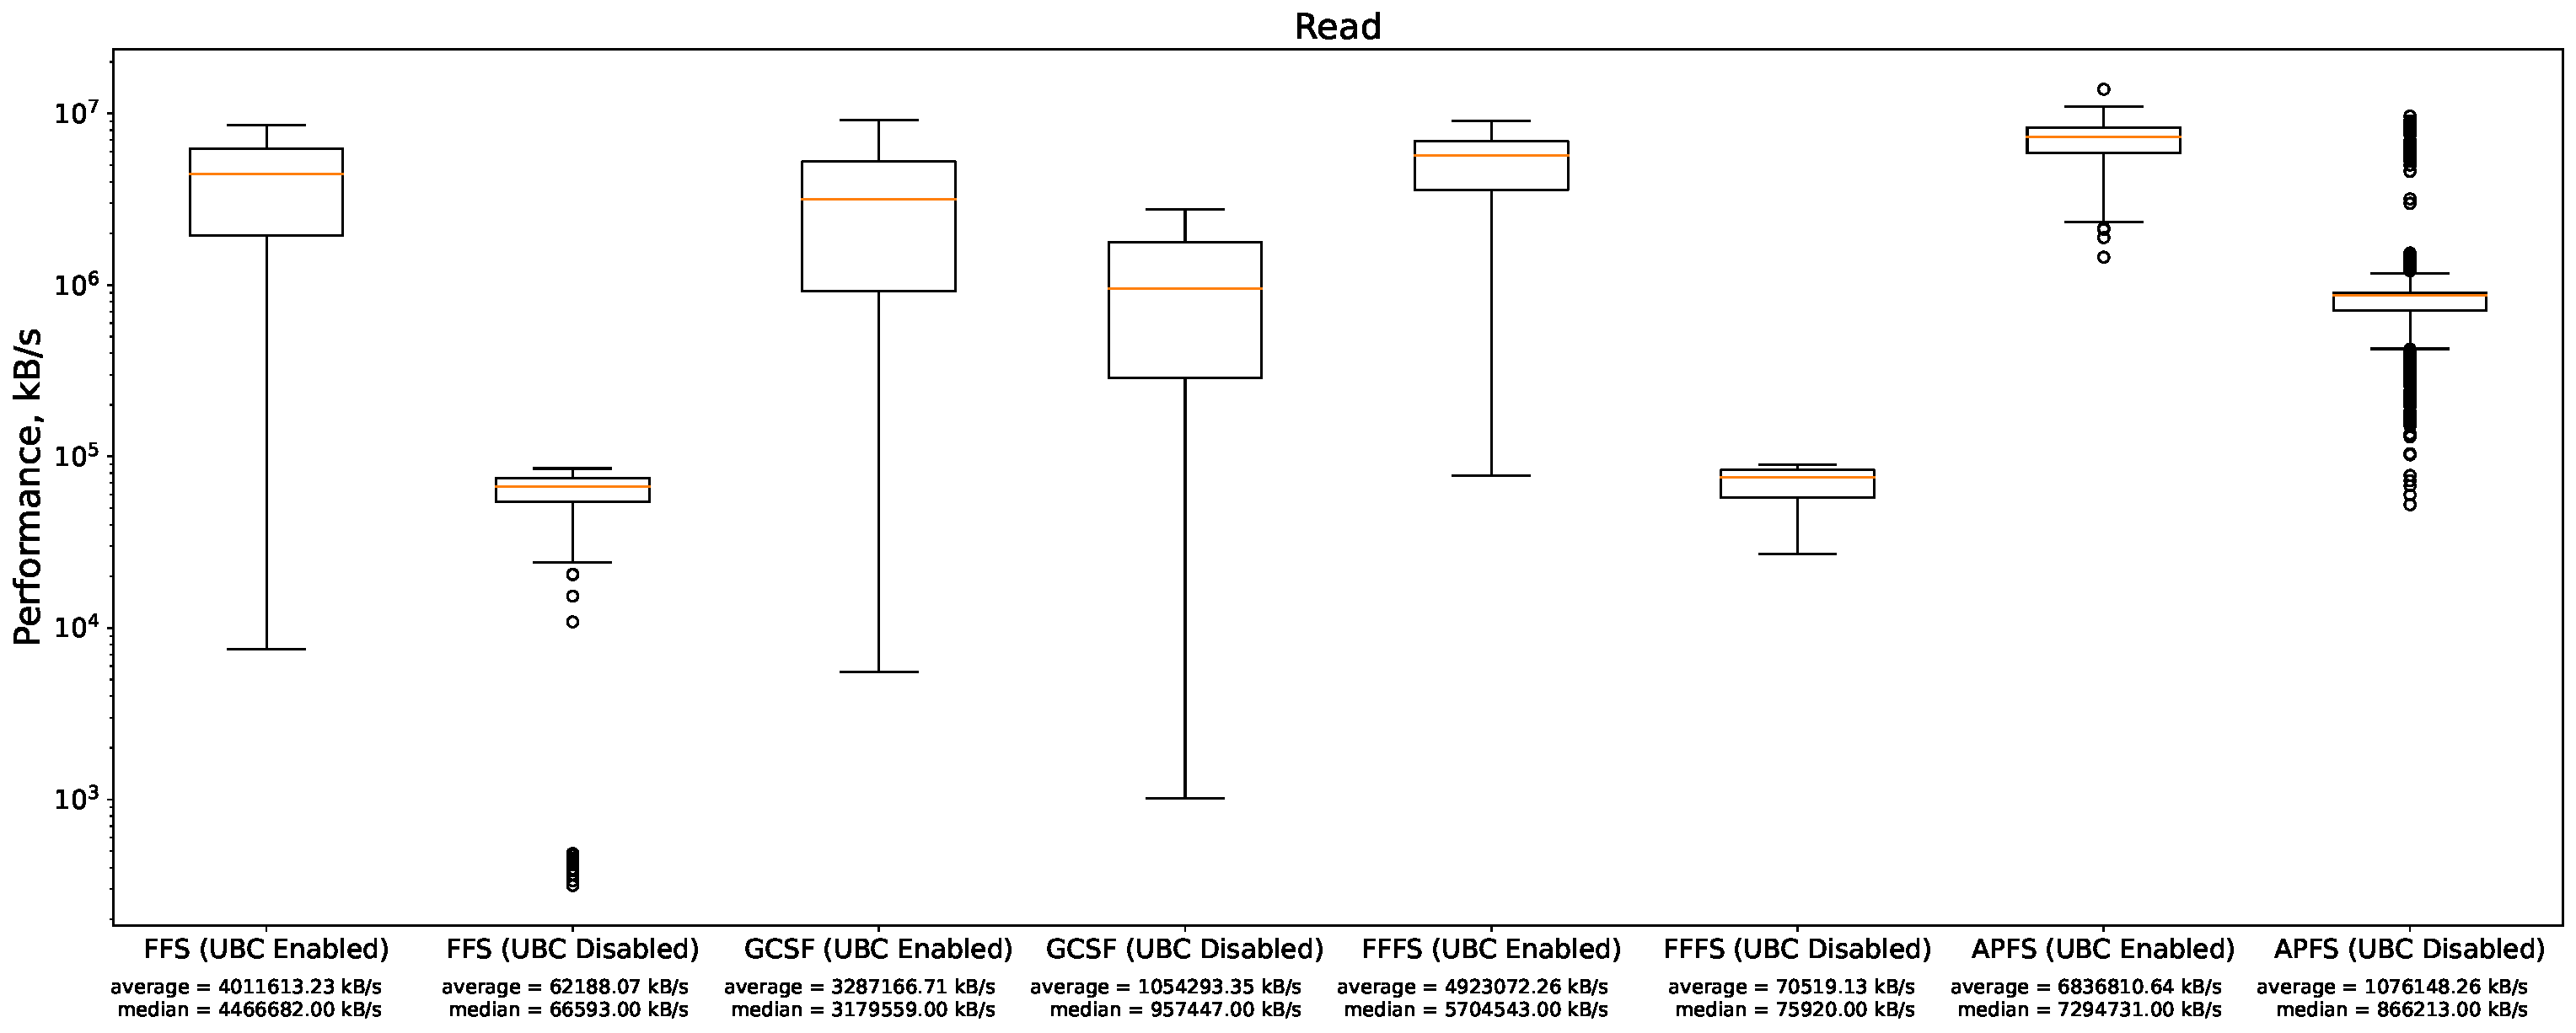
\includegraphics[width=1.0\textwidth]{figures.nosync/benchmarking/Read-boxplot.pdf}
	\end{center}
	\caption{Box plot of the IOZone output for the Read test on the different filesystems}
\end{figure}

\FloatBarrier

Figure~\ref{fig:res_box_write} presents a box plot of the benchmarking results of the filesystems of the Write test. \gls{APFS} has the best write performance of the four filesystems, both when the \gls{UBC} is enabled and when it is disabled. \gls{FFFS} performs better than the \mbox{cloud-based} filesystems for both states of the \gls{UBC}. \gls{FFFS} and \gls{GCSF} have similar performance when the \gls{UBC} is enabled and when it is disabled, while \gls{FFS} and \gls{APFS} perform significantly better with the \gls{UBC} enabled.

\begin{figure}[!ht]
	\label{fig:res_box_write}
	\begin{center}
		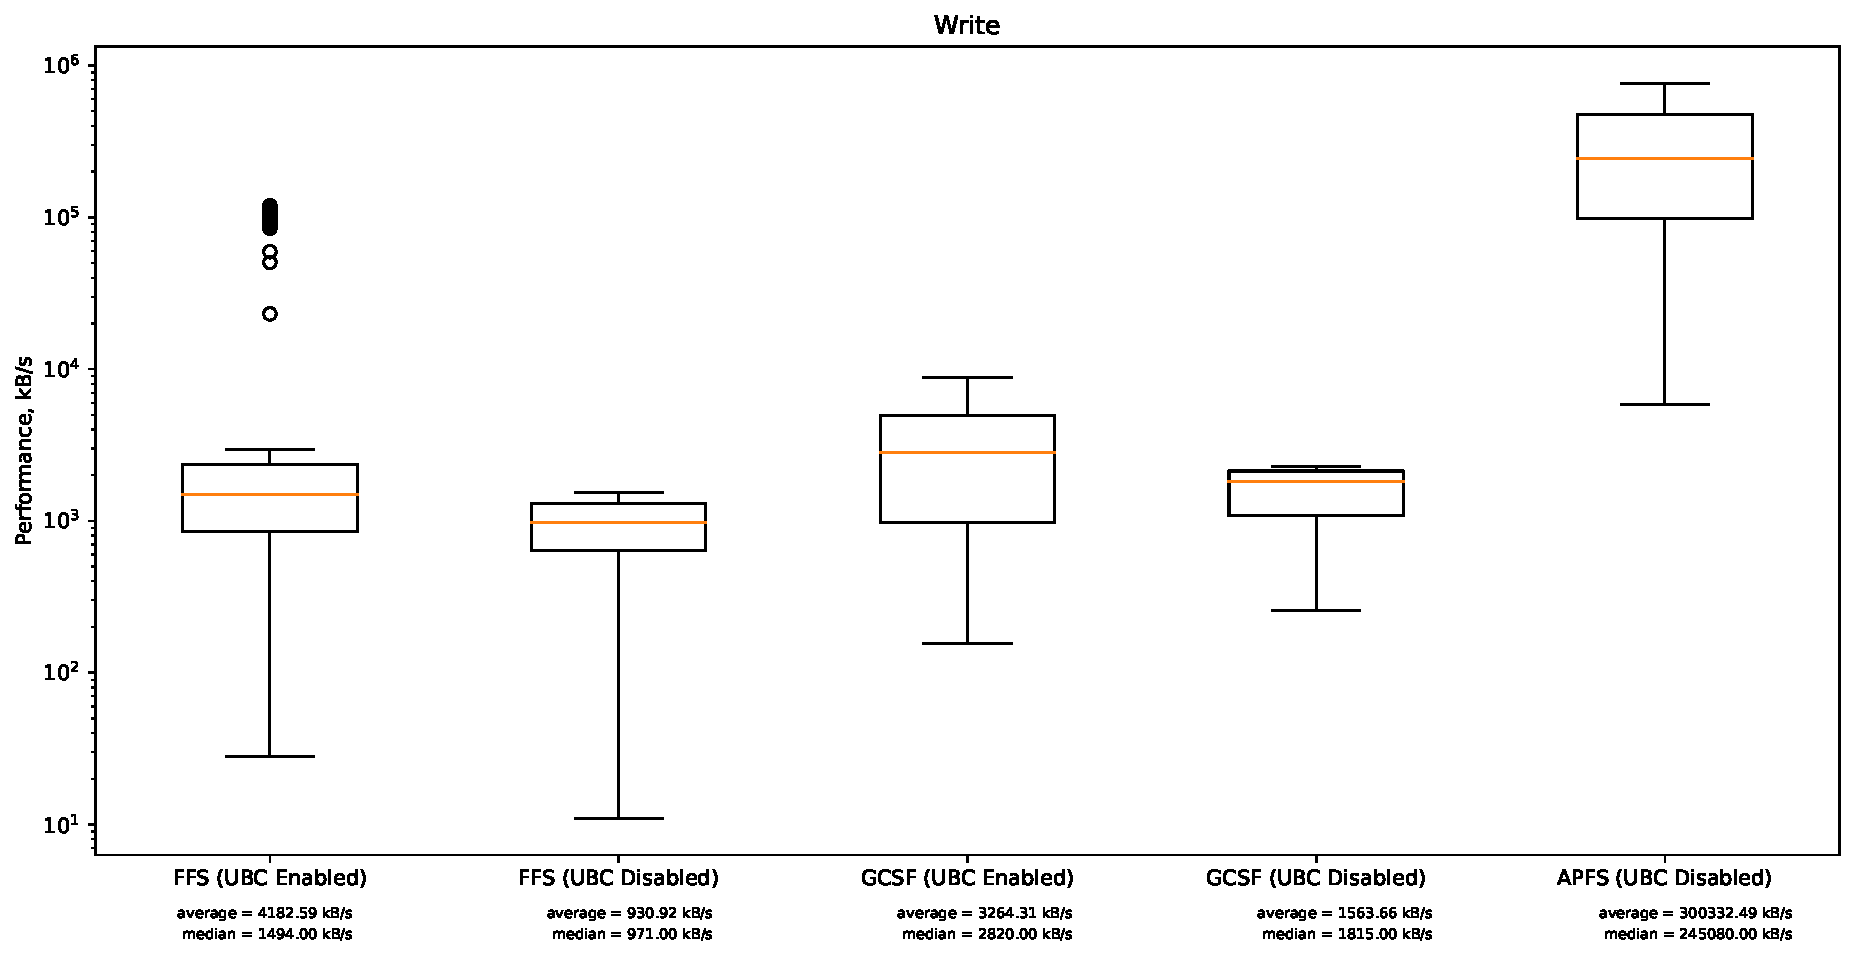
\includegraphics[width=1.0\textwidth]{figures.nosync/benchmarking/Write-boxplot.pdf}
	\end{center}
	\caption{Box plot of the IOZone output for the Write test on the different filesystems}
\end{figure}

\FloatBarrier

Figure~\ref{fig:res_box_reread} presents the result of the \mbox{Re-Read} test for the filesystems. \gls{FFS}, \gls{GCSF}, and \gls{FFFS} perform significantly better with the \gls{UBC} enabled compared to when it is disabled. \gls{APFS} also performs better with the \gls{UBC} enabled, but the performance difference compared to when the \gls{UBC} is disabled is not as large as for the other filesystems. When the \gls{UBC} is disabled, \gls{GCSF} performs better than \gls{FFS} and \gls{FFFS}. Although, when the \gls{UBC} is disabled, \gls{GCSF} has a greater spread of values with its worst performance being lower than the worst performance of \gls{FFS} and \gls{FFFS} when the \gls{UBC} is disabled.

\begin{figure}[!ht]
	\label{fig:res_box_reread}
	\begin{center}
		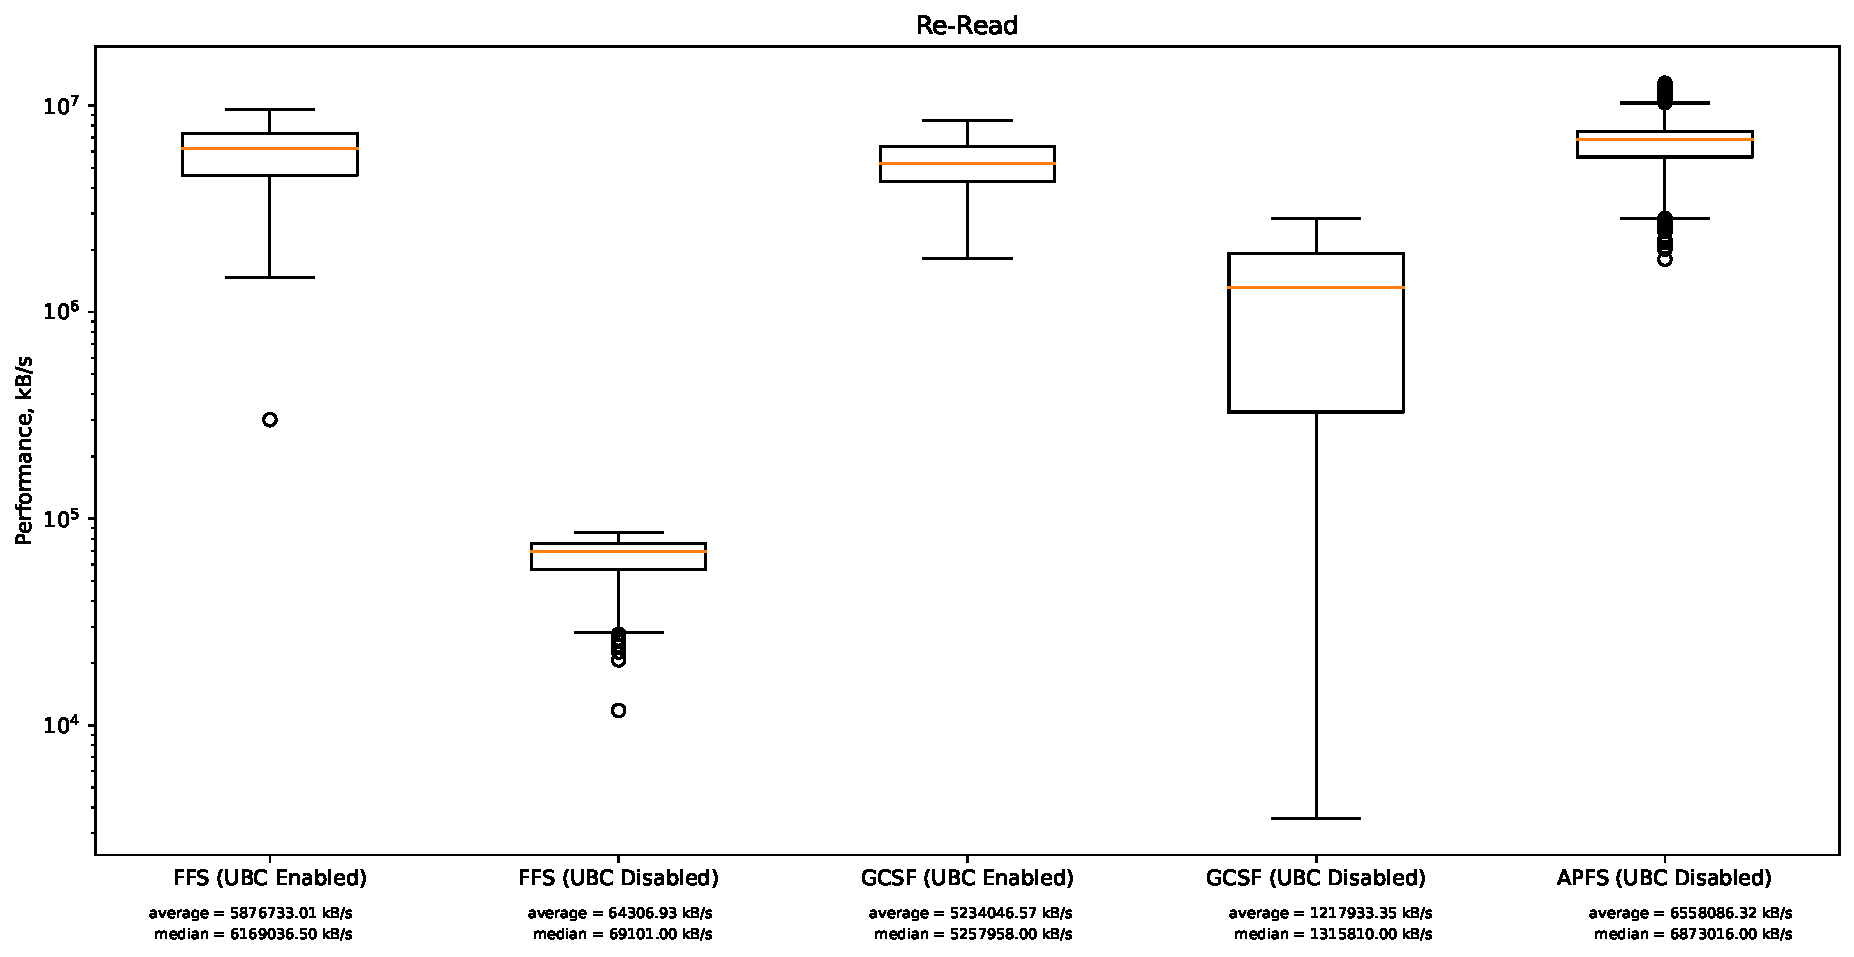
\includegraphics[width=1.0\textwidth]{figures.nosync/benchmarking/Re-Read-boxplot.pdf}
	\end{center}
	\caption{Box plot of the IOZone output for the Re-Read test on the different filesystems}
\end{figure}

\FloatBarrier

Figure~\ref{fig:res_box_rewrite} presents a box plot for the \mbox{Re-Write} test for the filesystems. 

Similar to the Write test results presented in Figure~\ref{fig:res_box_write}, \gls{APFS} has the best performance of the filesystems, both when the \gls{UBC} is enabled and when it is disabled. \gls{FFFS} performs better than the \mbox{cloud-based} filesystems for both states of the \gls{UBC}. \gls{FFS} has slightly better average performance compared to \gls{GCSF} when the \gls{UBC} is enabled, but worse median performance. \gls{GCSF} has better average and median performance than \gls{FFS} when the \gls{UBC} is disabled.

\begin{figure}[!ht]
	\label{fig:res_box_rewrite}
	\begin{center}
		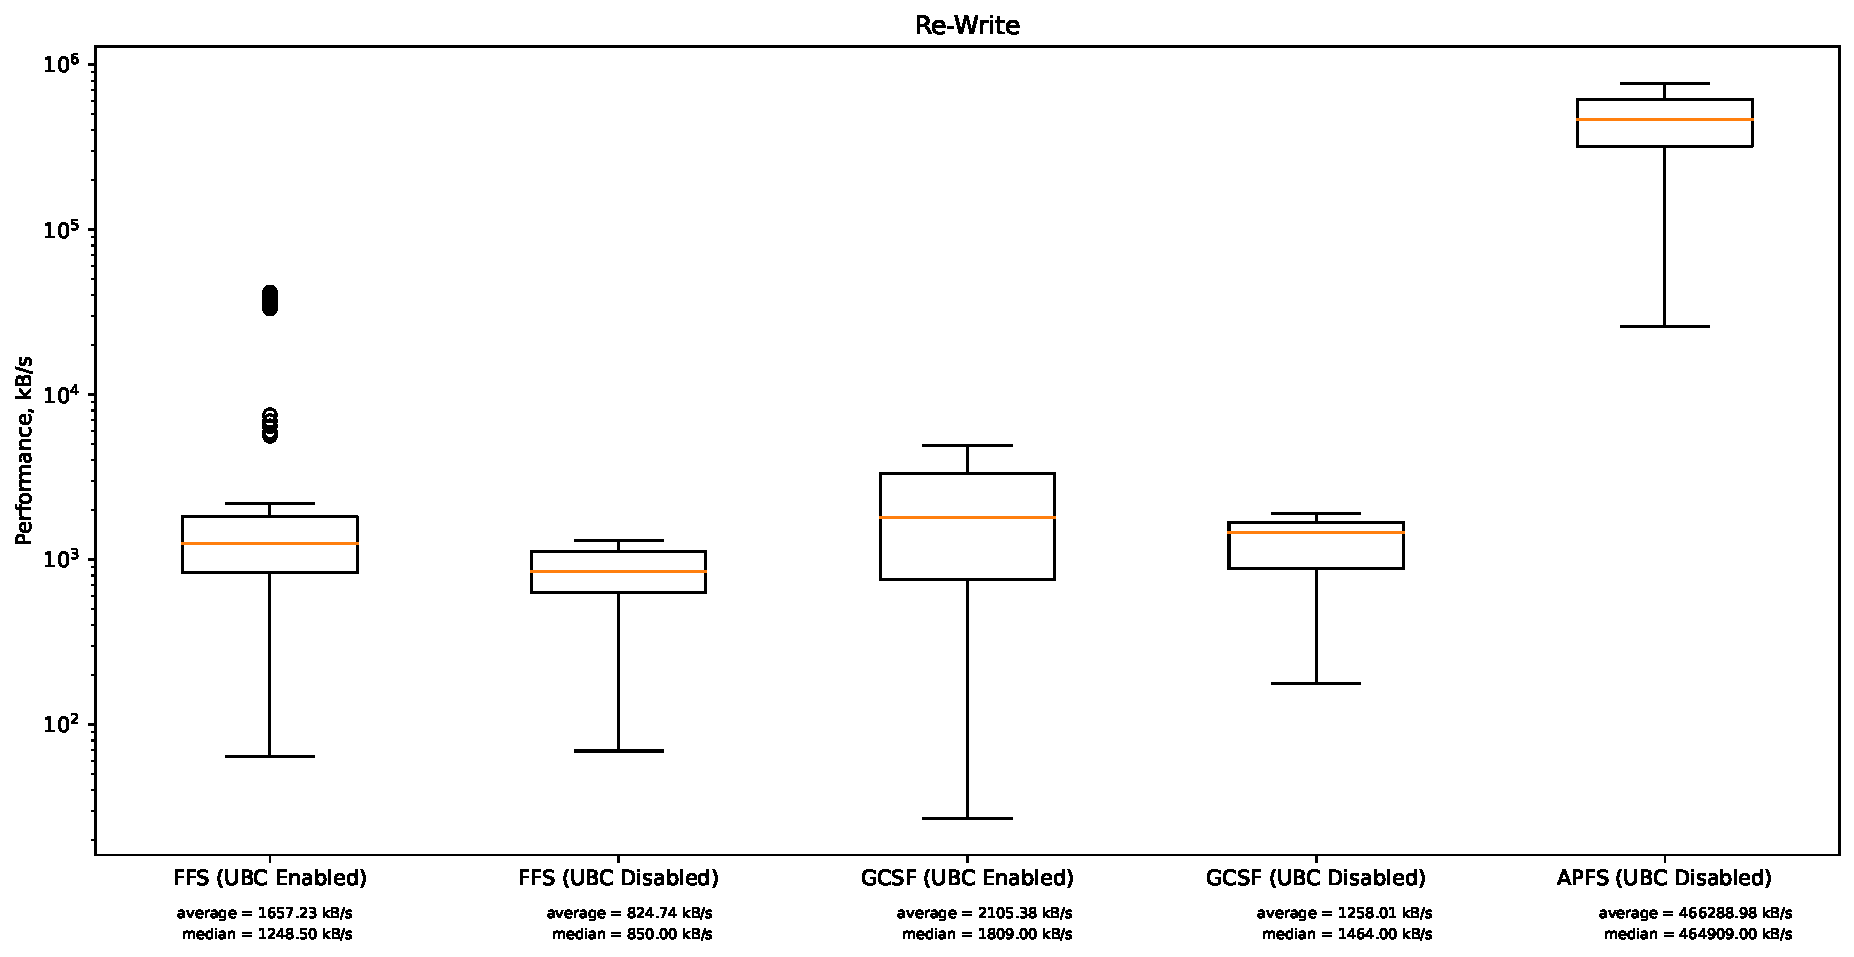
\includegraphics[width=1.0\textwidth]{figures.nosync/benchmarking/Re-Write-boxplot.pdf}
	\end{center}
	\caption{Box plot of the IOZone output for the Re-Write test on the different filesystems}
\end{figure}

\FloatBarrier

Figure~\ref{fig:res_box_rndread} presents a box plot for the Random read test for the different filesystems. The results are similar to the results for the \mbox{Re-Read} test presented in Figure~\ref{fig:res_box_reread}.

\begin{figure}[!ht]
	\label{fig:res_box_rndread}
	\begin{center}
		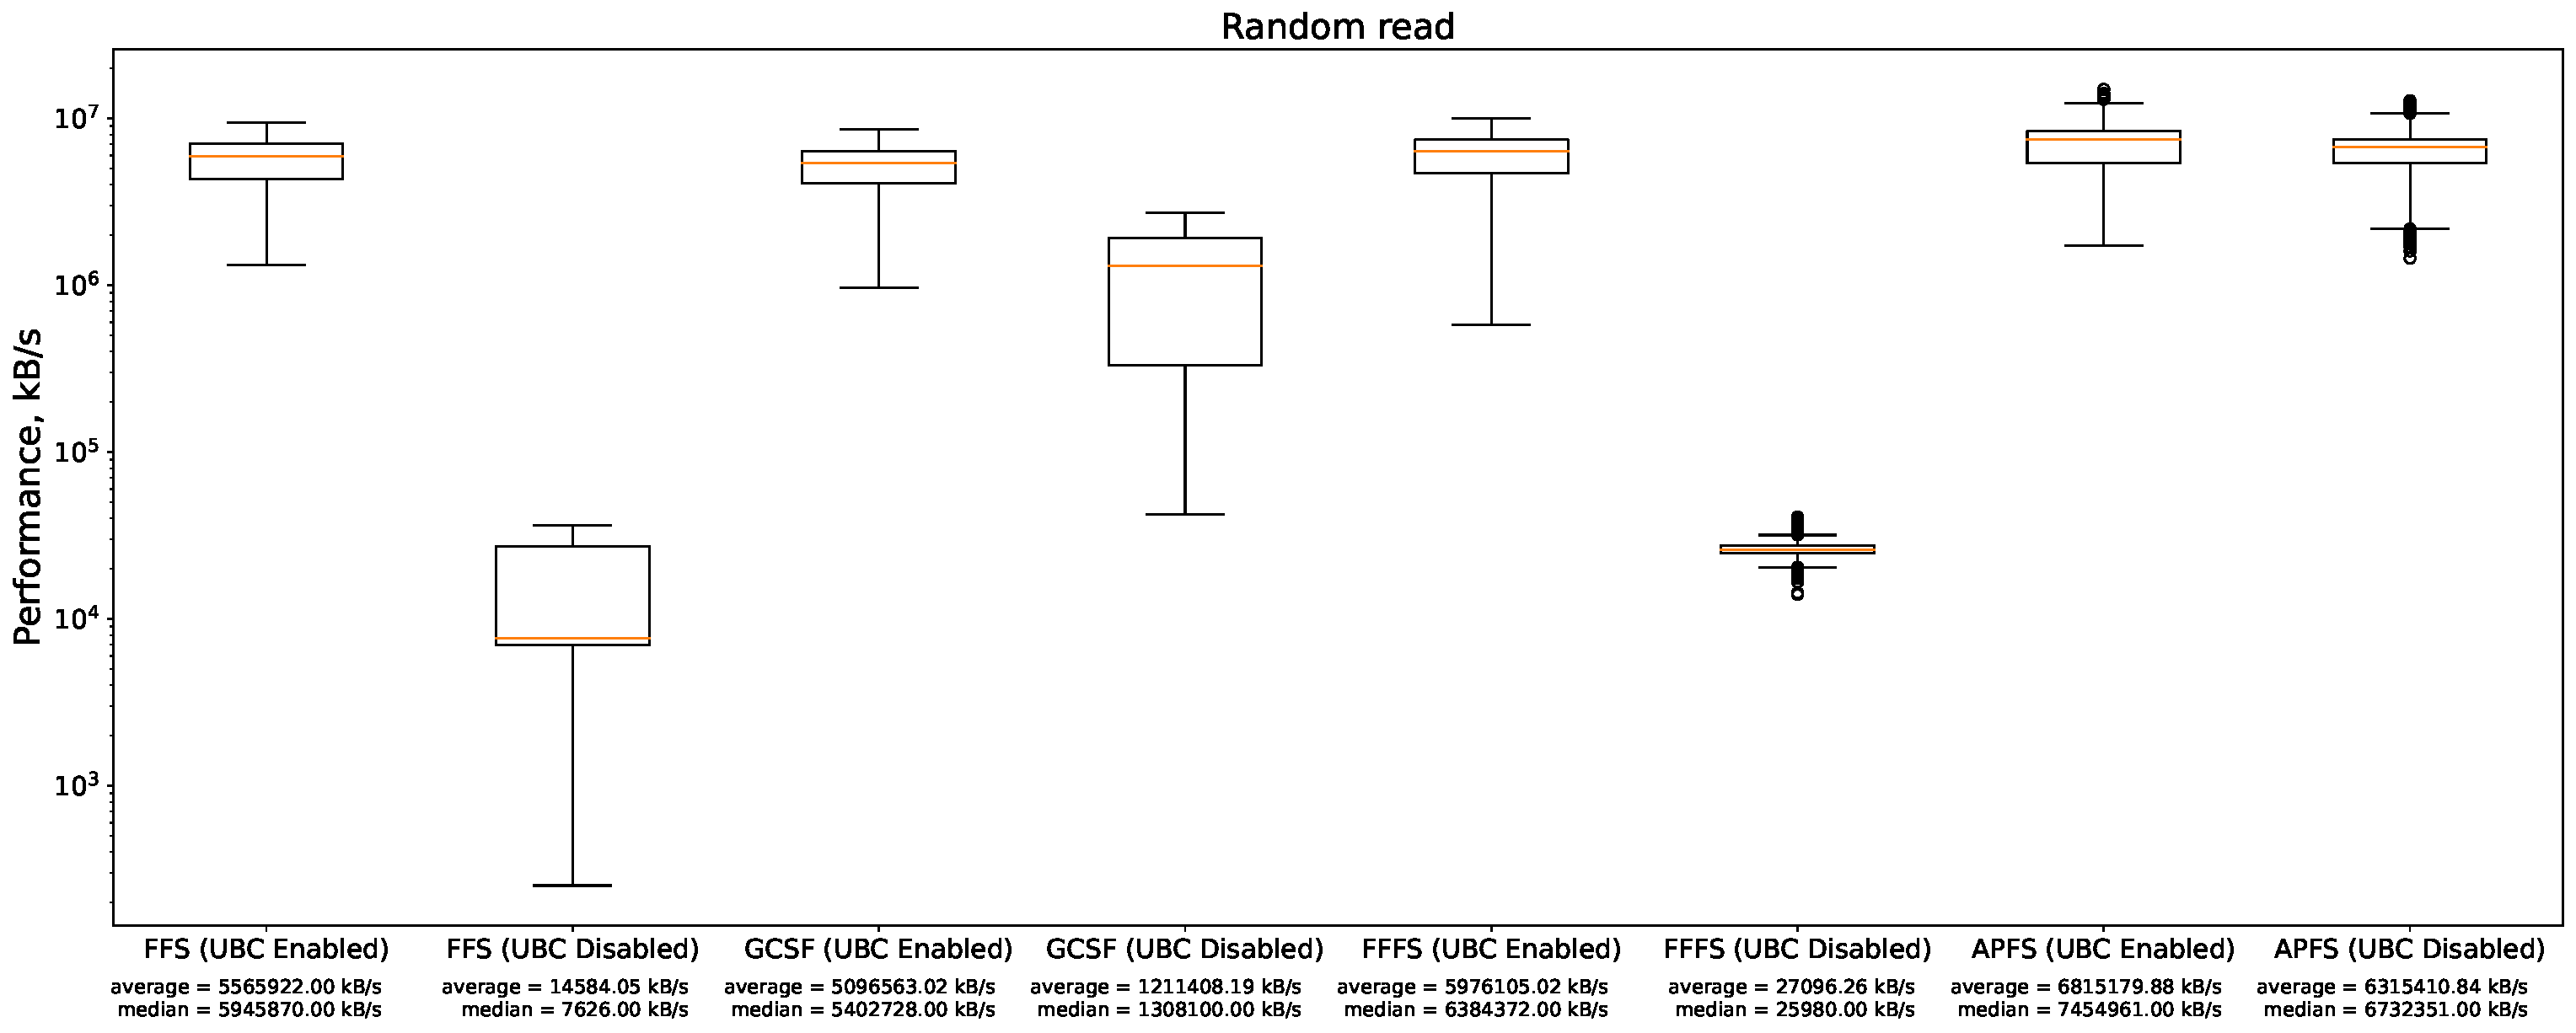
\includegraphics[width=1.0\textwidth]{figures.nosync/benchmarking/Random read-boxplot.pdf}
	\end{center}
	\caption{Box plot of the IOZone output for the Random read test on the different filesystems}
\end{figure}

\FloatBarrier

Figure~\ref{fig:res_box_rndwrite} presents a box plot for the Random read test for the different filesystems.The results are similar to the results for the \mbox{Re-Write} test presented in Figure~\ref{fig:res_box_rewrite}.

\begin{figure}[!ht]
	\label{fig:res_box_rndwrite}
	\begin{center}
		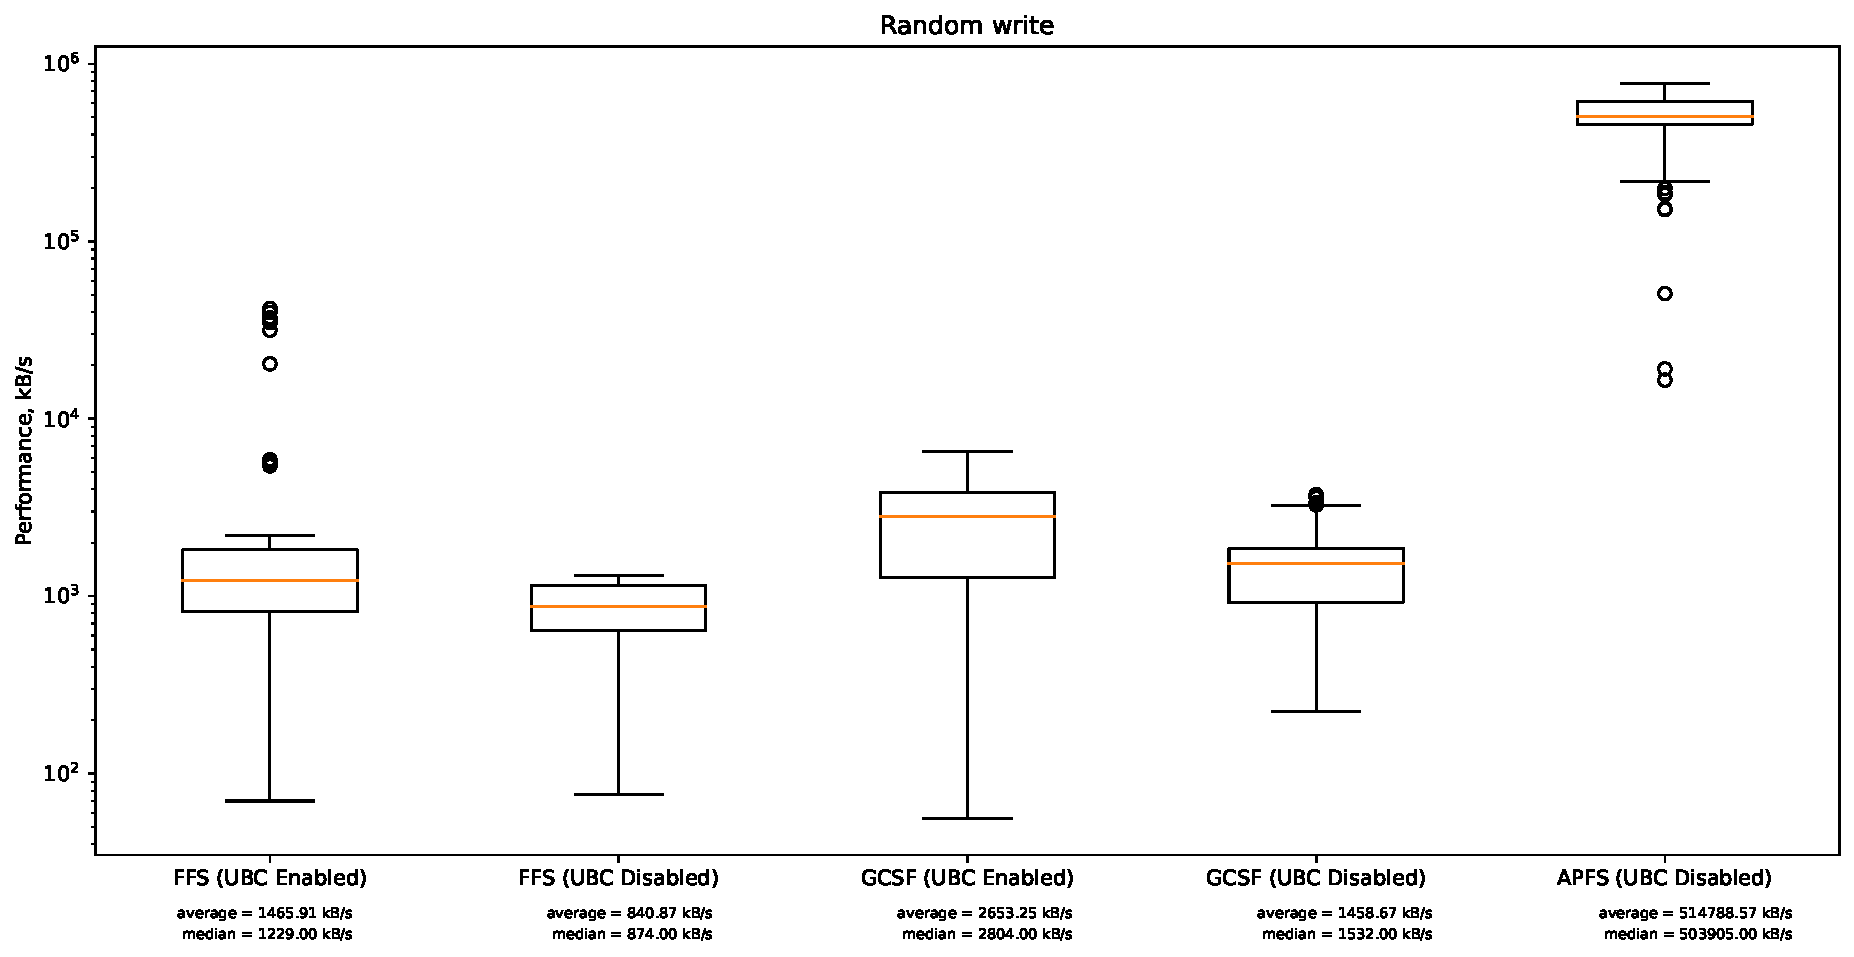
\includegraphics[width=1.0\textwidth]{figures.nosync/benchmarking/Random write-boxplot.pdf}
	\end{center}
	\caption{Box plot of the IOZone output for the Random write test on the different filesystems}
\end{figure}

\FloatBarrier

Following are histograms for each filesystem and each state of the \gls{UBC}. Each histogram presents the performance distribution for each file size in each file operation test. Figure~\ref{fig:bench_ffs_with_cache} and Figure~\ref{fig:bench_ffs_without_cache} presents the performance of \gls{FFS} with the \gls{UBC} enabled and disabled, respectively. Figure~\ref{fig:bench_gcsf_with_cache} and Figure~\ref{fig:bench_gcsf_without_cache} presents the performance of \gls{GCSF} with the \gls{UBC} enabled and disabled, respectively. Figure~\ref{fig:bench_fffs_with_cache} and Figure~\ref{fig:bench_fffs_without_cache} presents the performance of \gls{FFFS} with the \gls{UBC} enabled and disabled, respectively. Figure~\ref{fig:bench_apfs_with_cache} and Figure~\ref{fig:bench_apfs_without_cache} presents the performance of \gls{APFS} with the \gls{UBC} enabled and disabled, respectively.

\begin{figure}[!htb]
	\label{fig:bench_ffs_with_cache}
	\begin{center}
		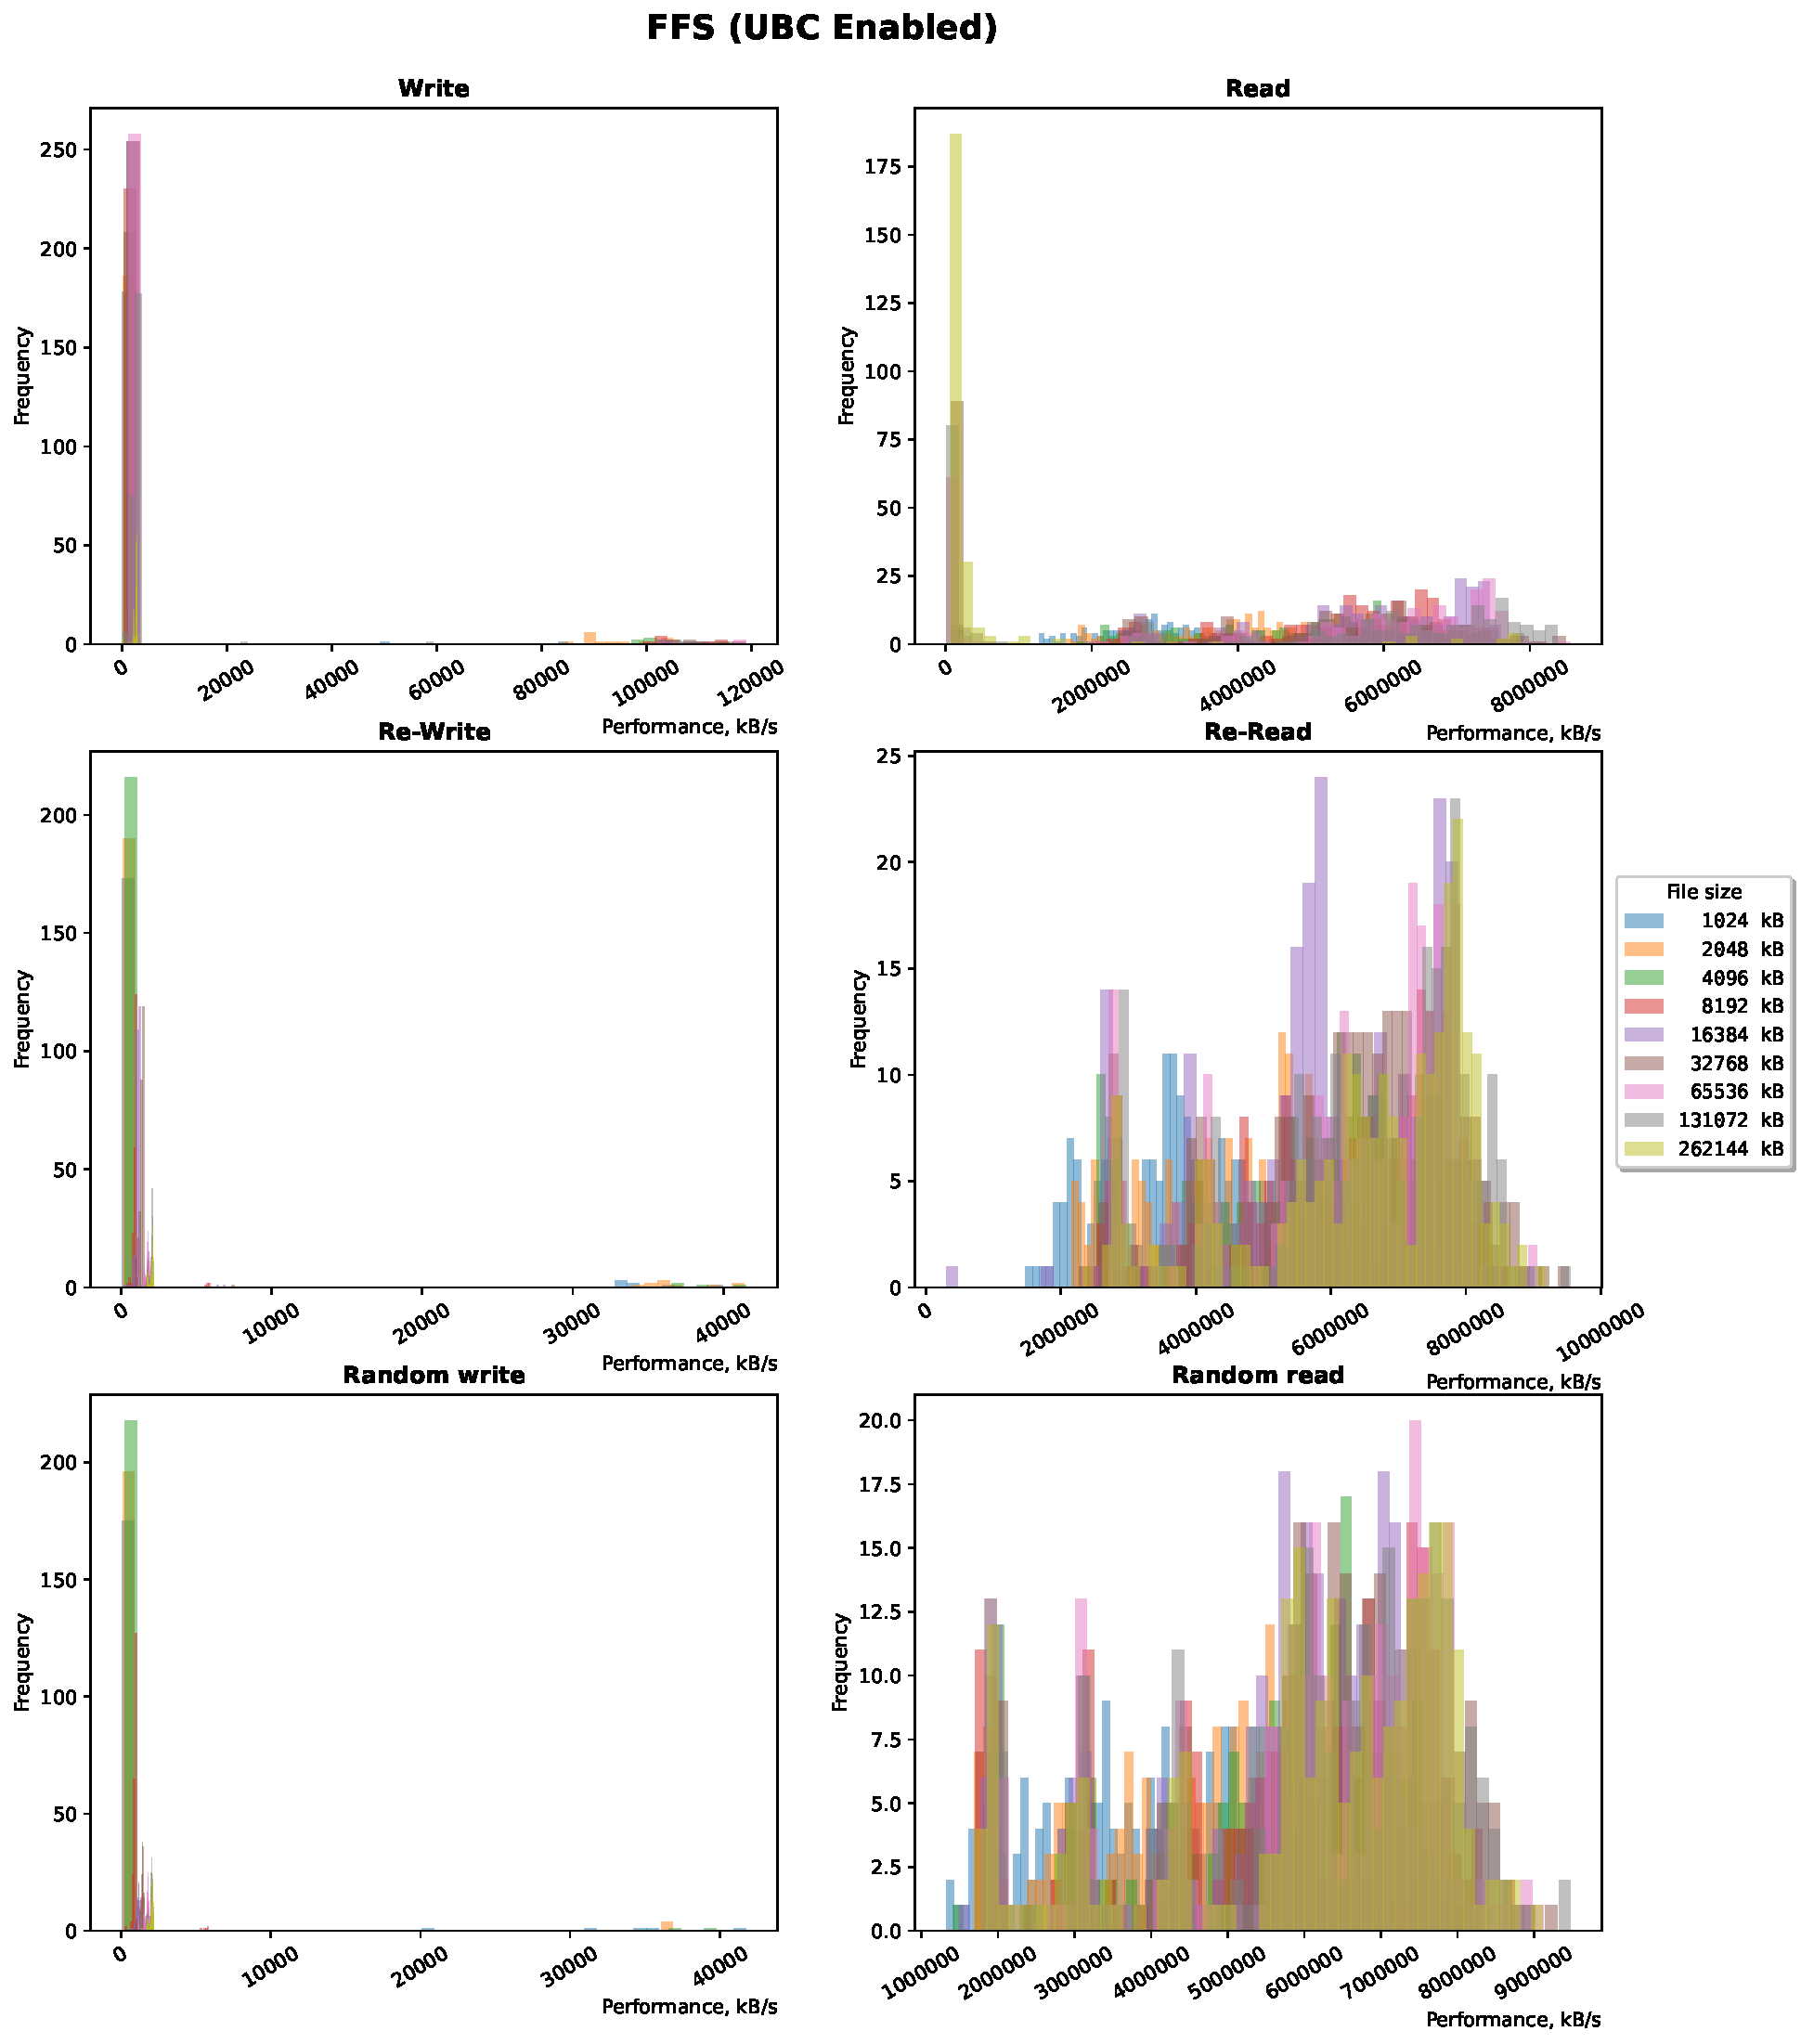
\includegraphics[width=1.0\textwidth]{figures.nosync/benchmarking/FFS/FFS-UBC Enabled-hist.pdf}
	\end{center}
	\caption{Performance comparison of different file sizes for FFS with the UBC enabled}
\end{figure}

\begin{figure}[!htb]
	\label{fig:bench_ffs_without_cache}
	\begin{center}
		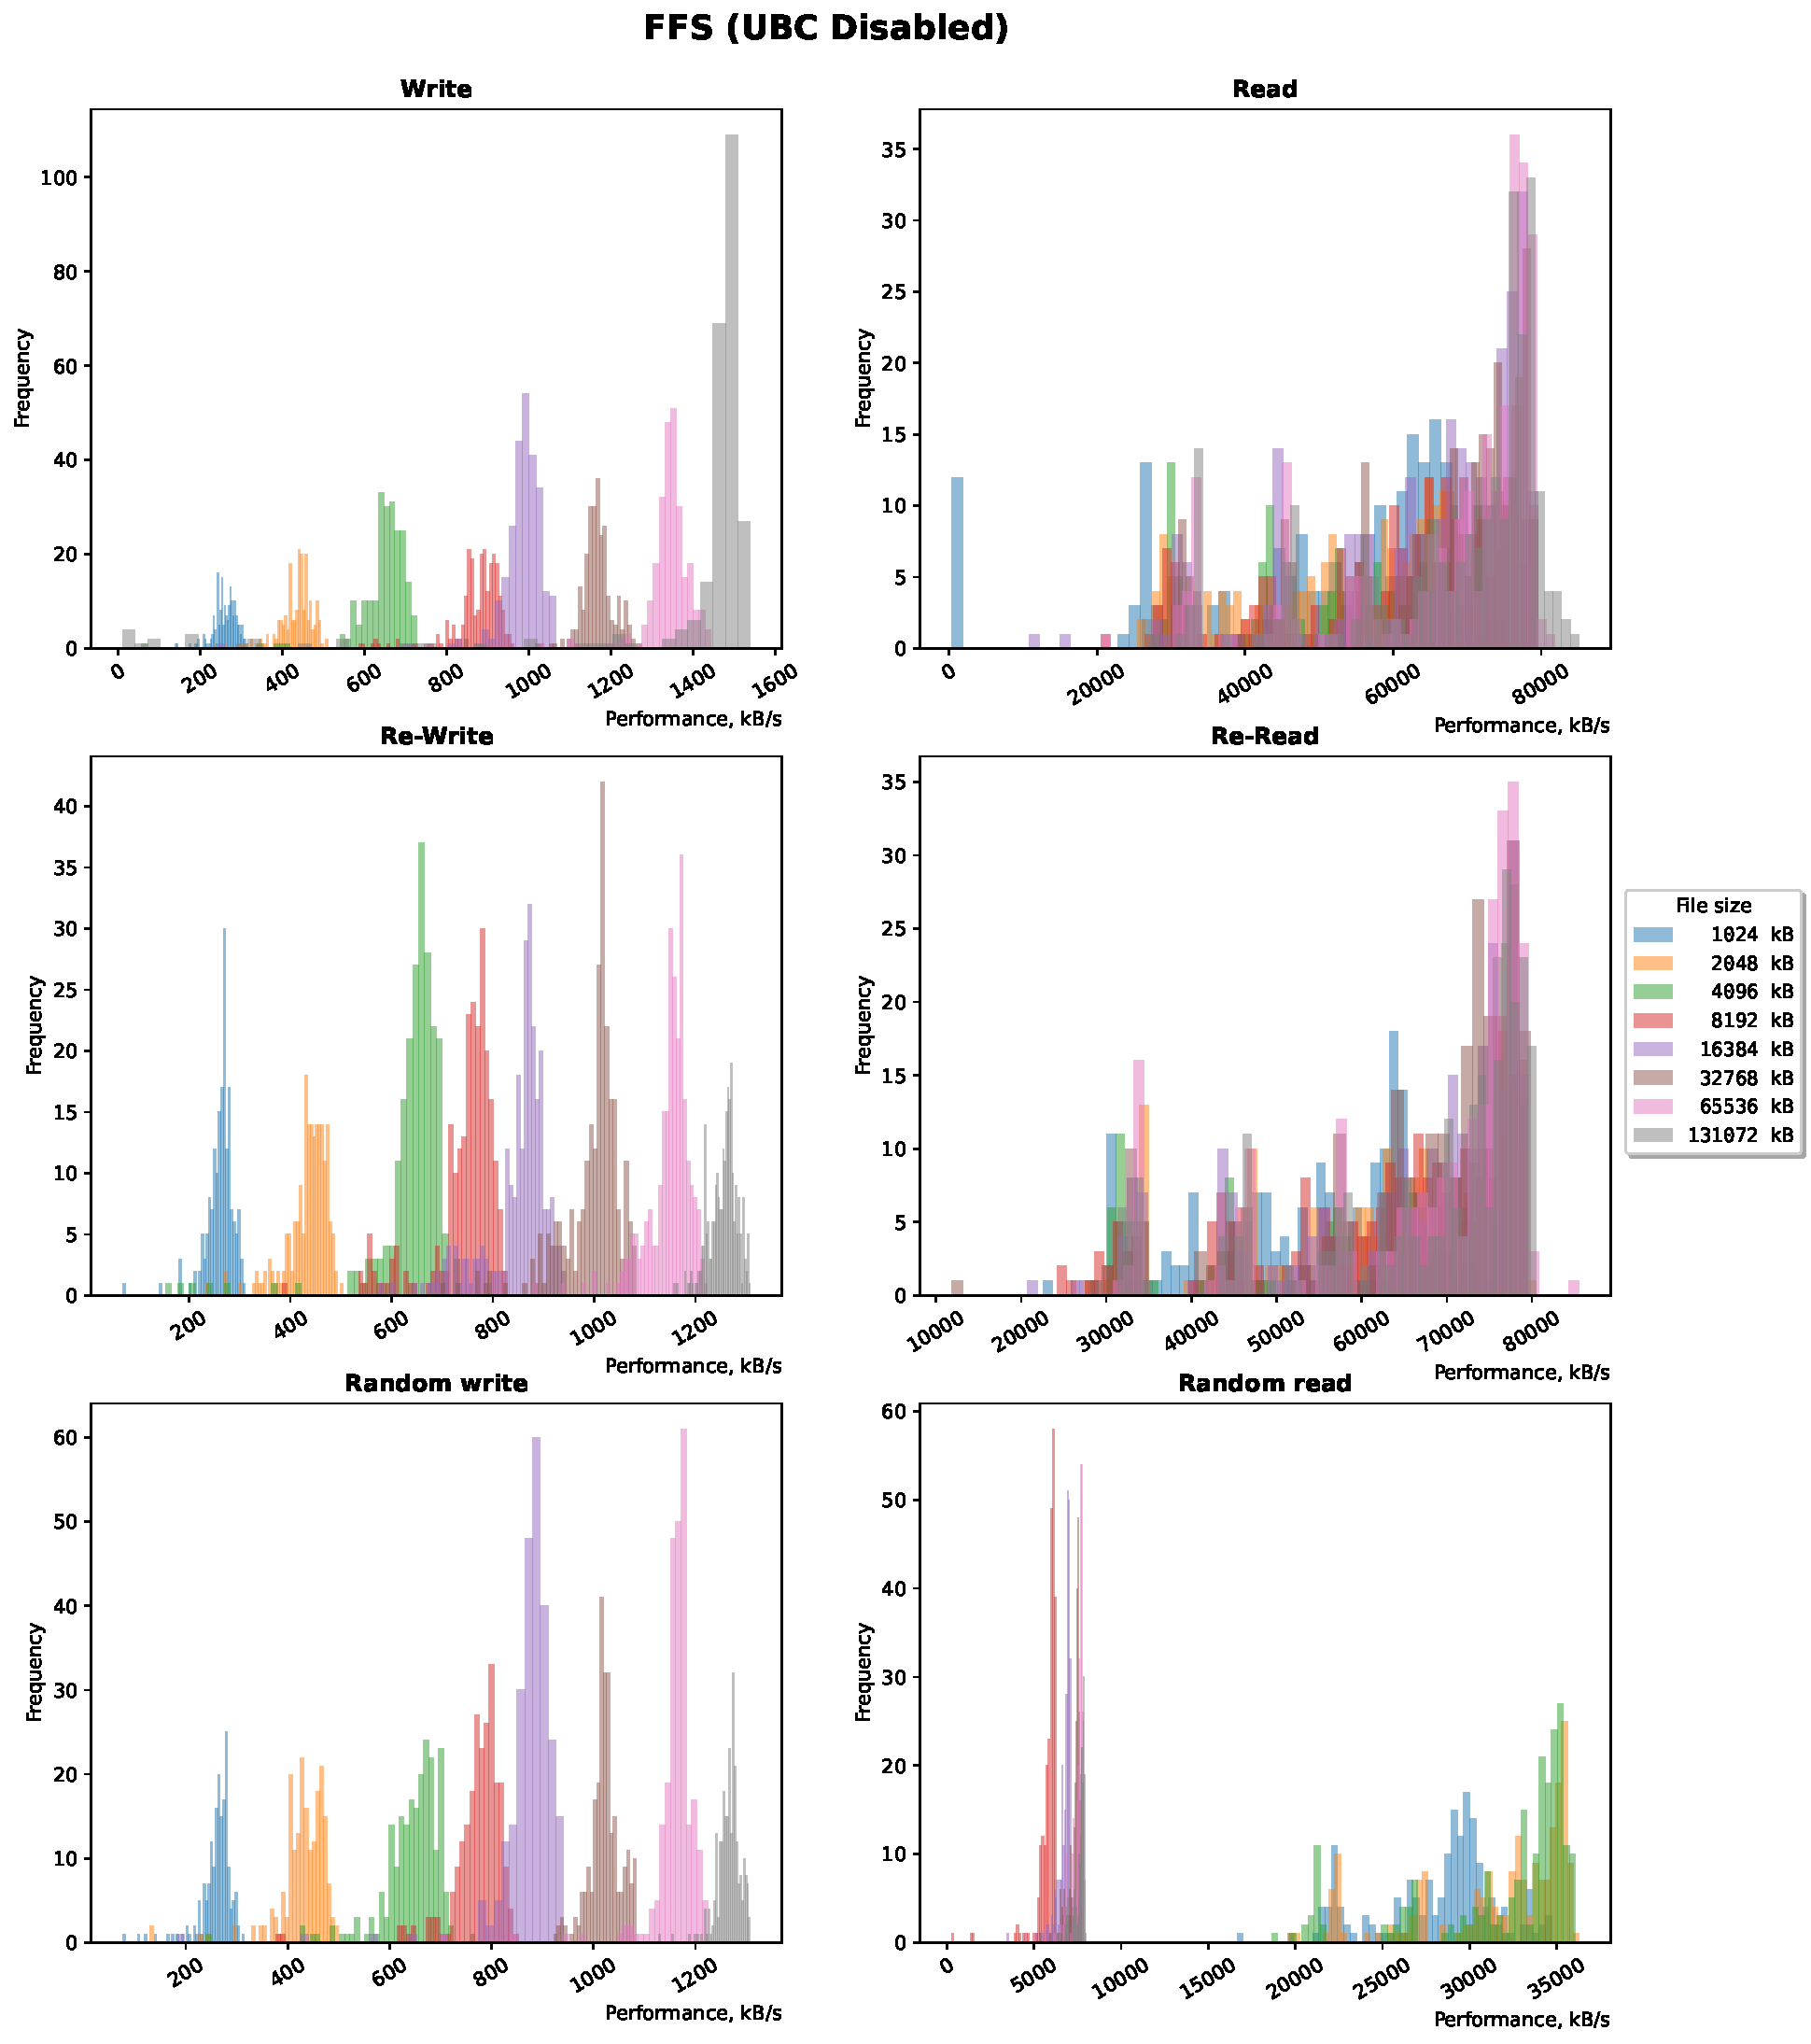
\includegraphics[width=1.0\textwidth]{figures.nosync/benchmarking/FFS/FFS-UBC Disabled-hist.pdf}
	\end{center}
	\caption{Performance comparison of different file sizes for FFS with the UBC disabled}
\end{figure}



\begin{figure}[!htb]
	\label{fig:bench_gcsf_with_cache}
	\begin{center}
		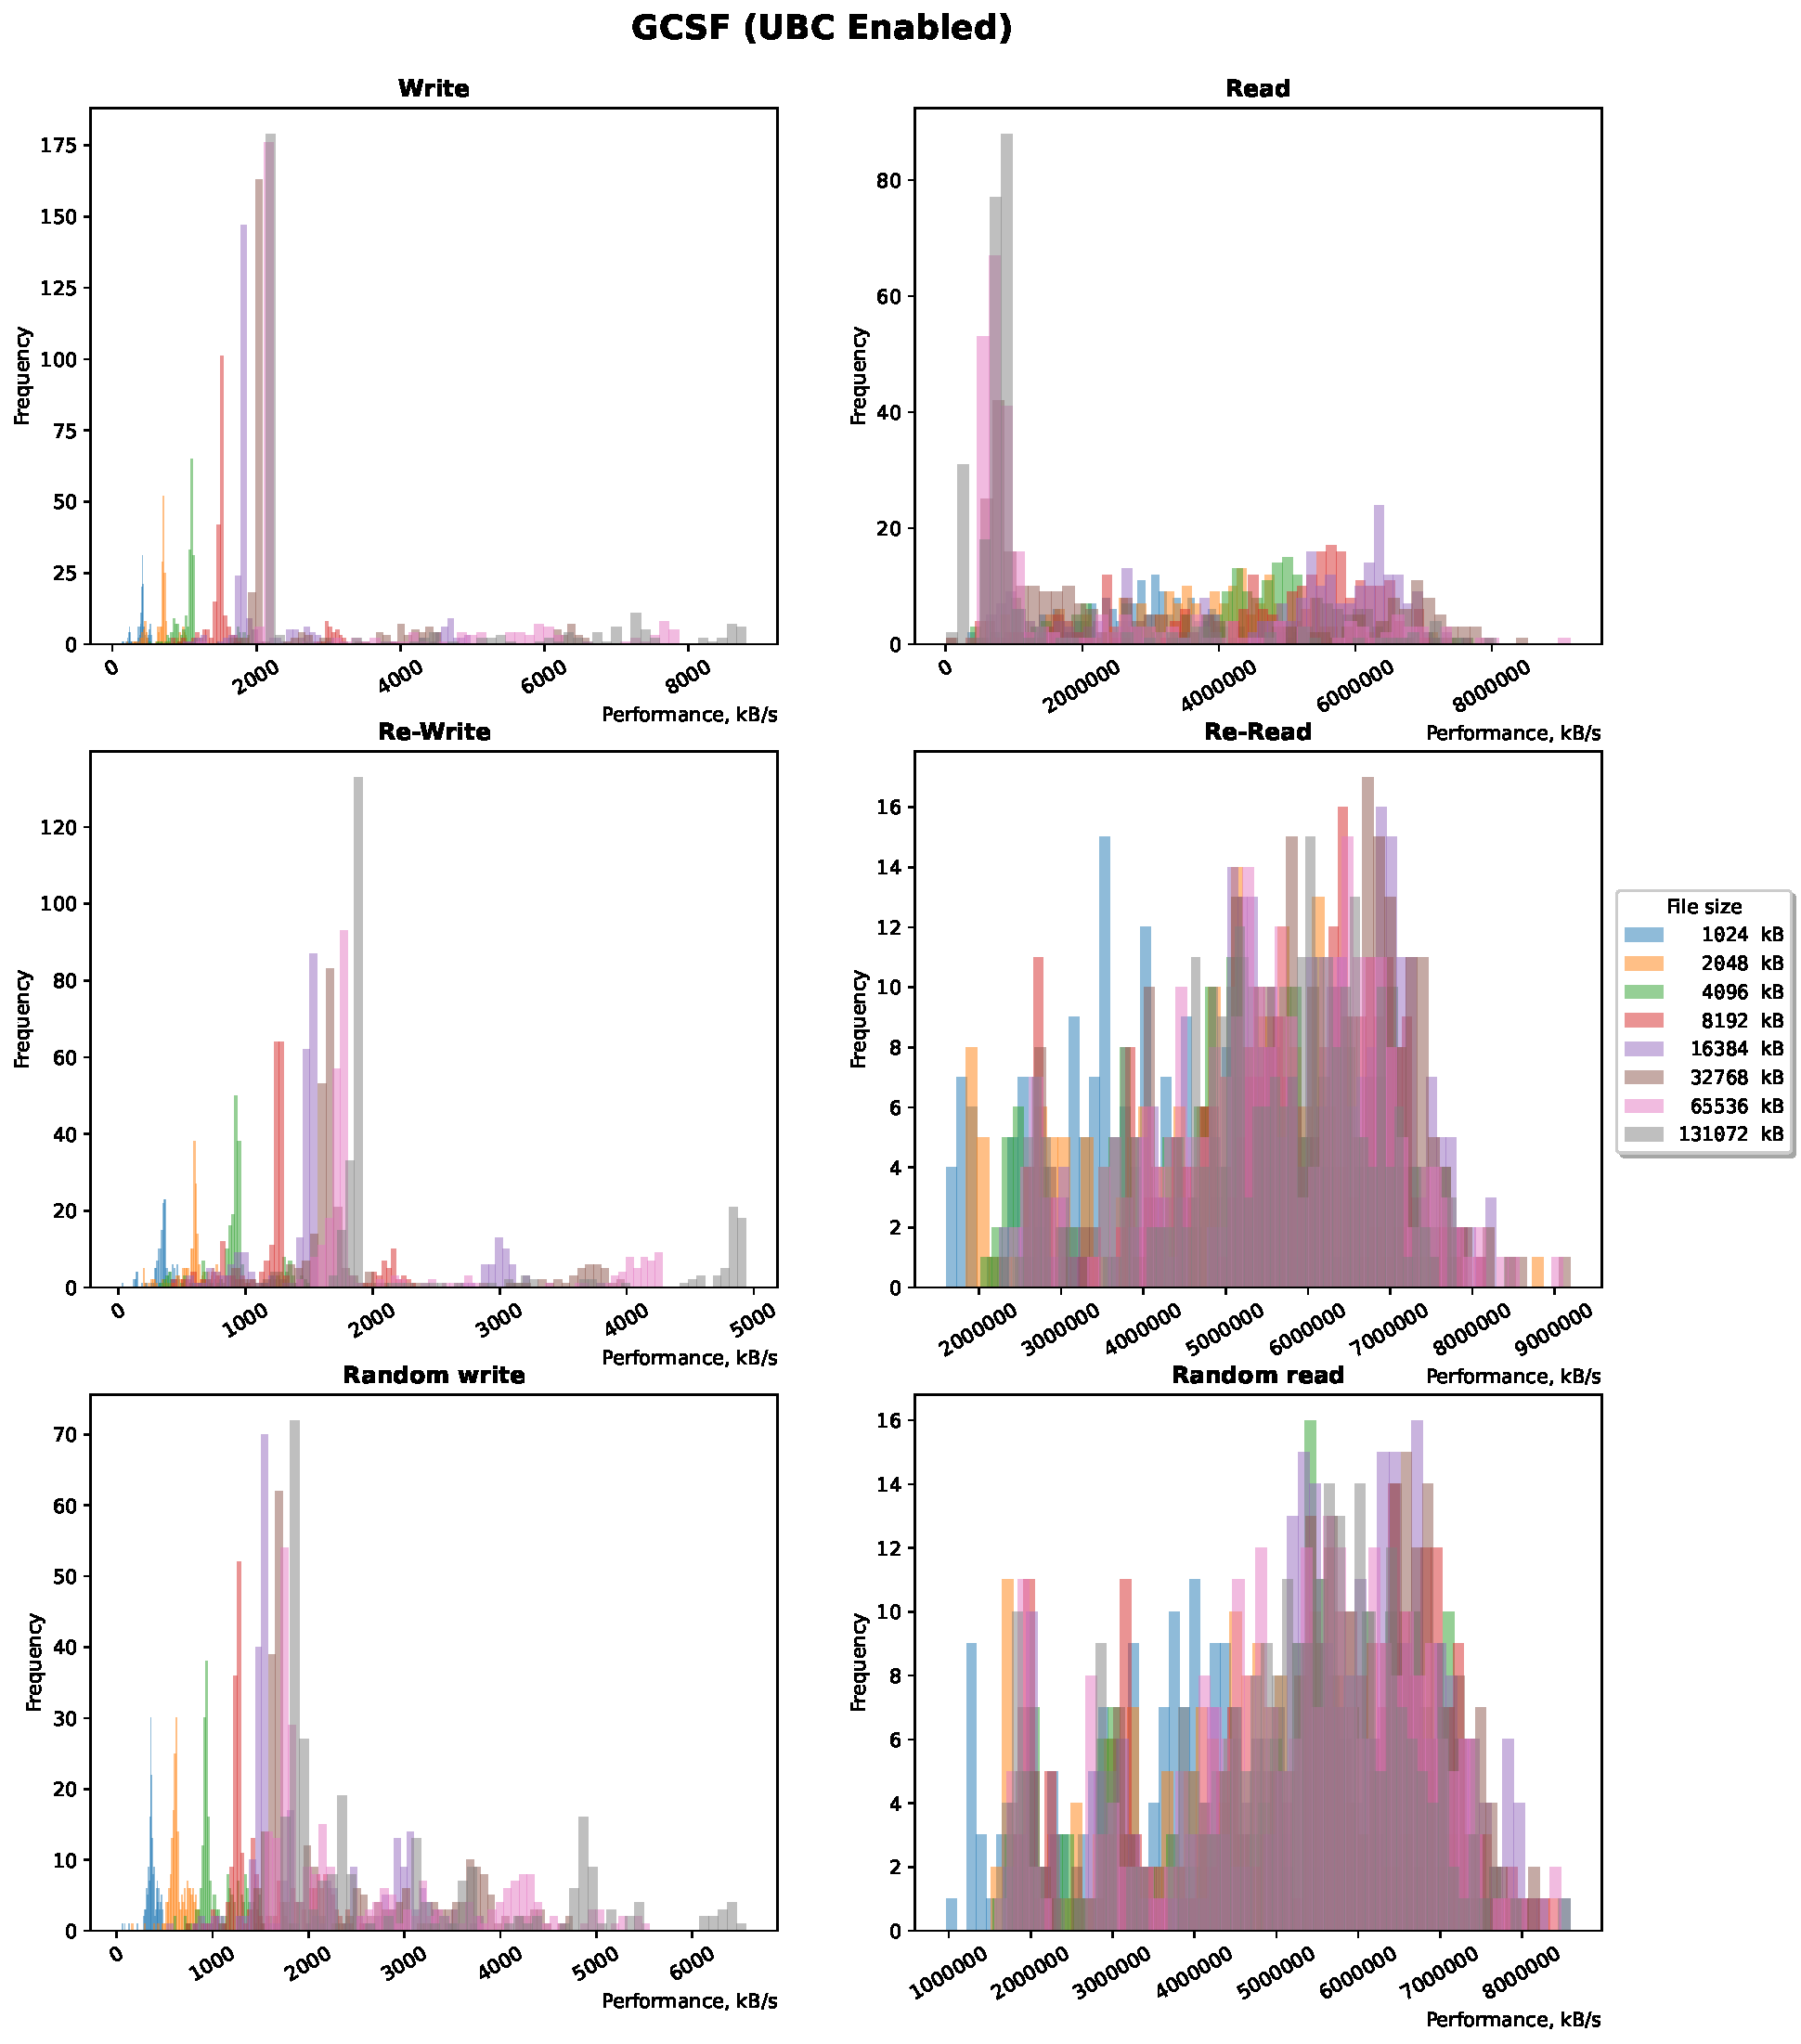
\includegraphics[width=1.0\textwidth]{figures.nosync/benchmarking/GCSF/GCSF-UBC Enabled-hist.pdf}
	\end{center}
	\caption{Performance comparison of different file sizes for GCSF with the UBC enabled}
\end{figure}

\begin{figure}[!htb]
	\label{fig:bench_gcsf_without_cache}
	\begin{center}
		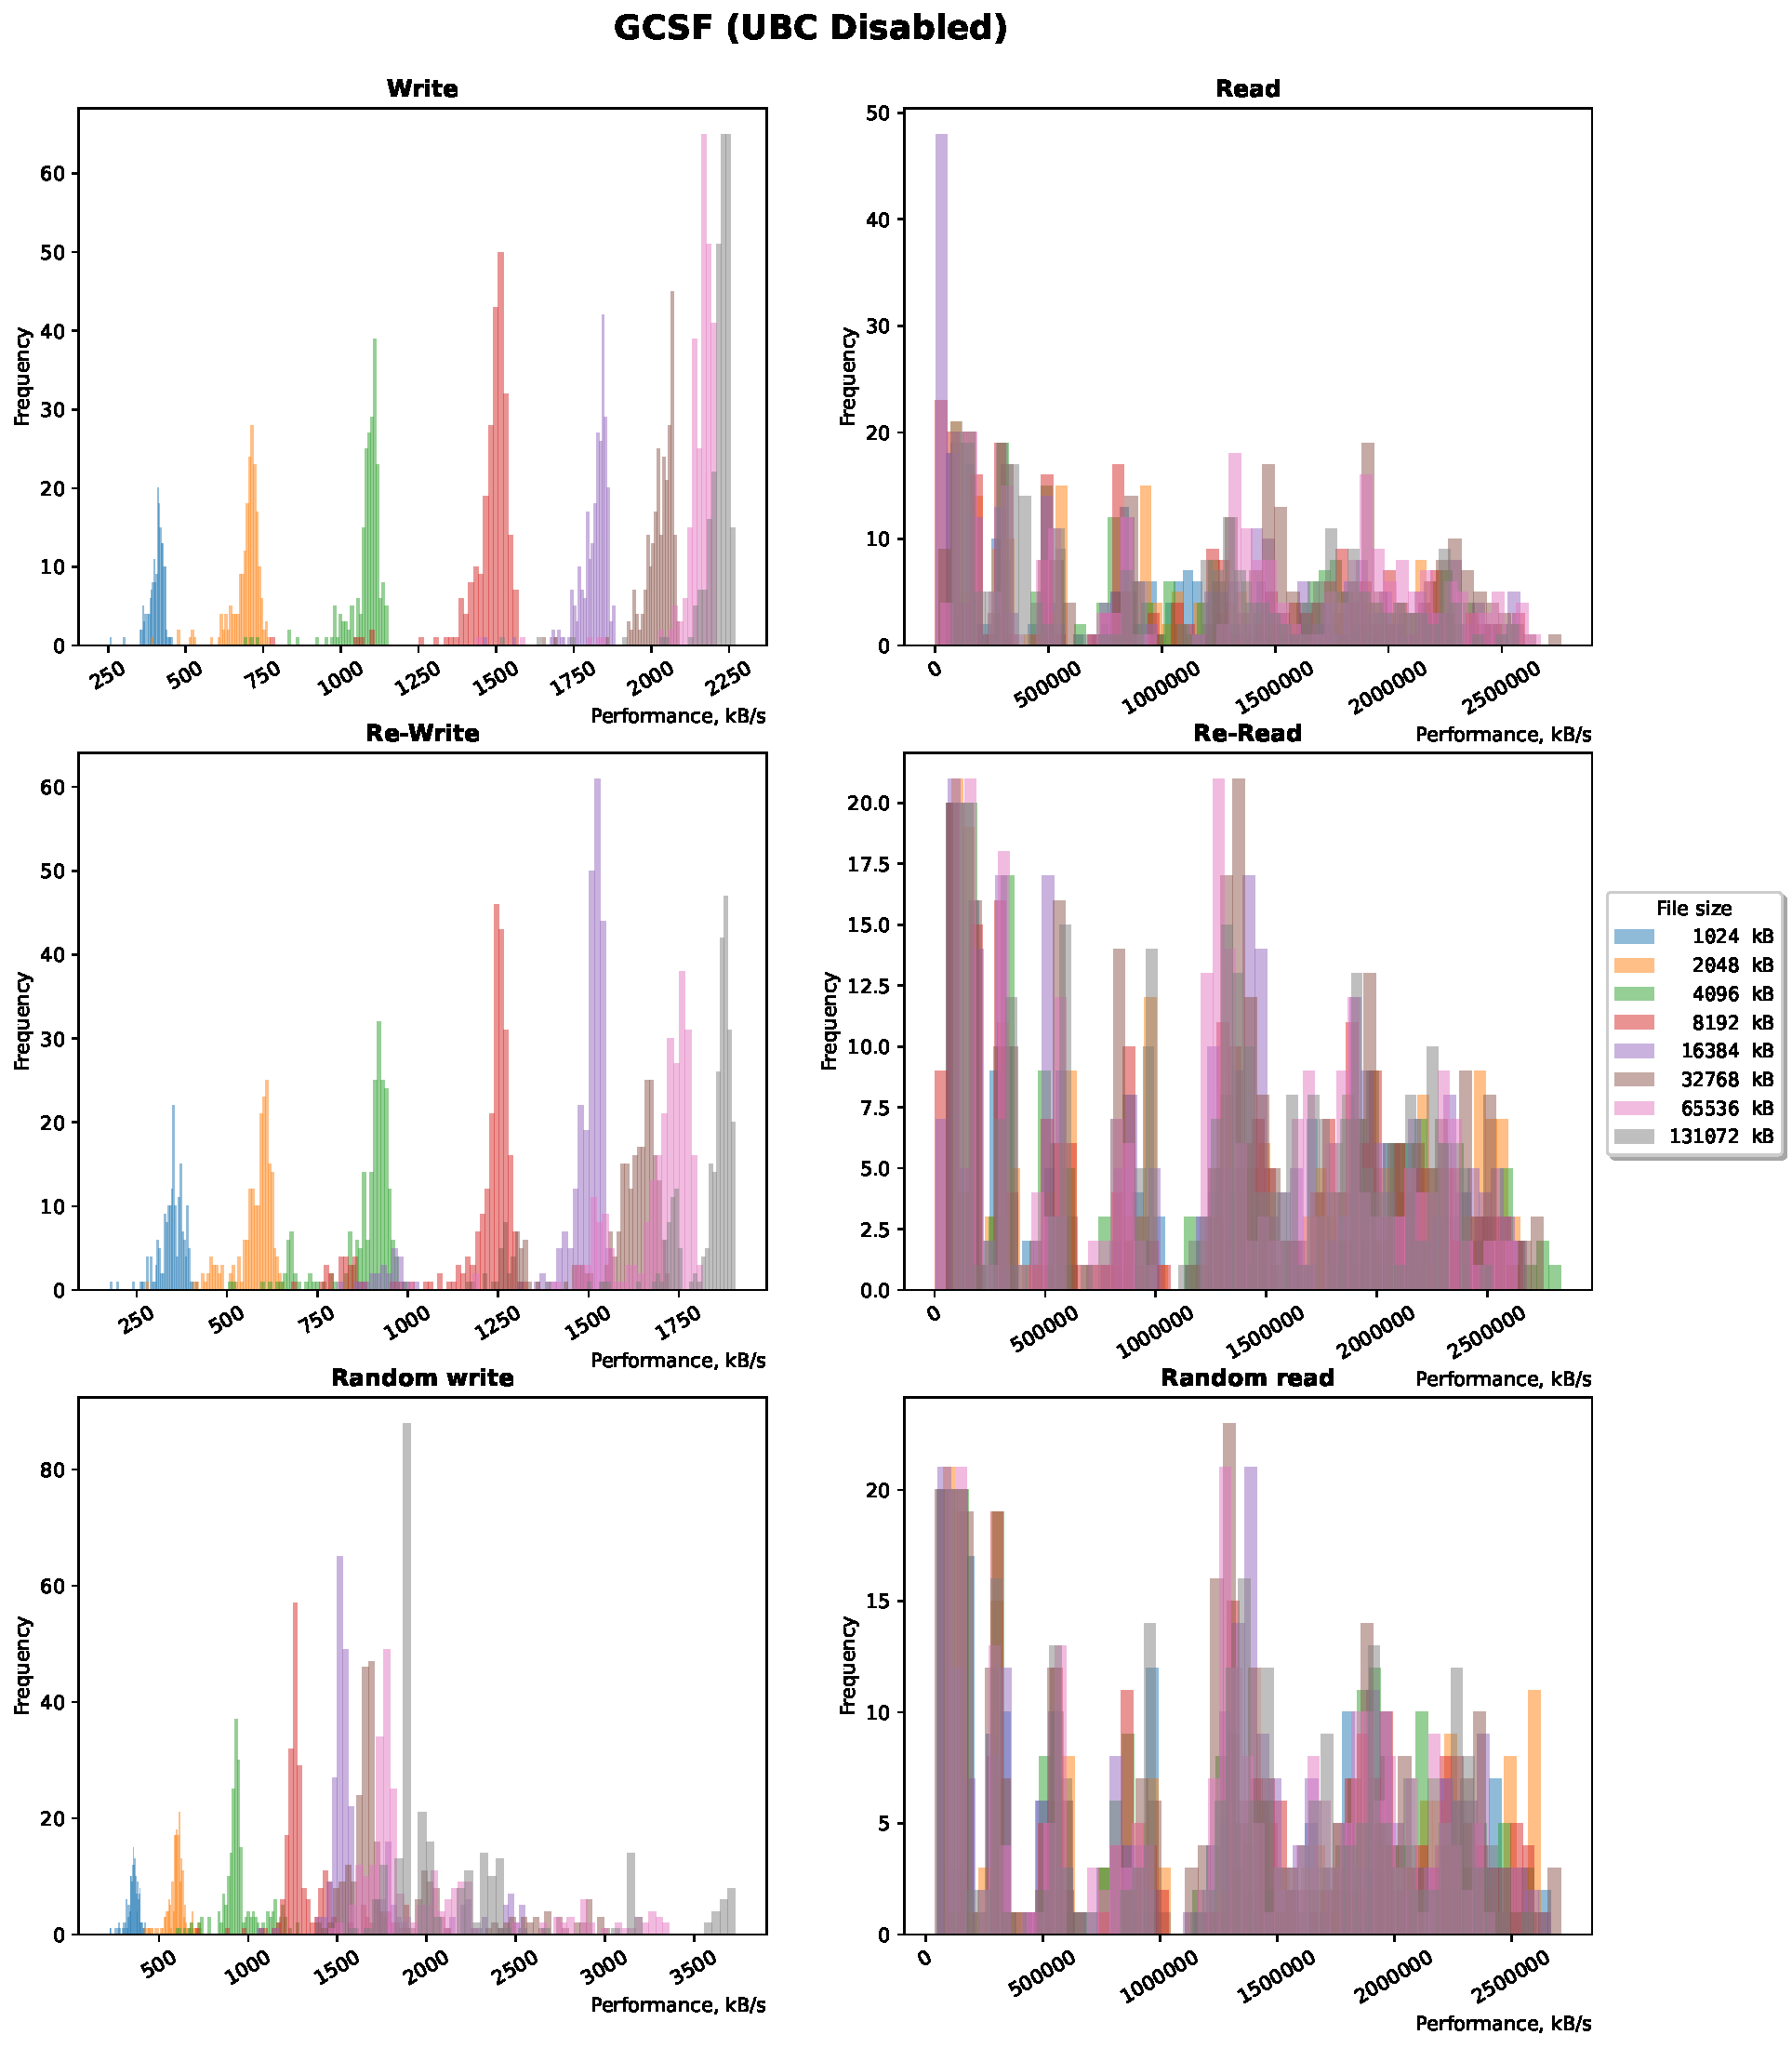
\includegraphics[width=1.0\textwidth]{figures.nosync/benchmarking/GCSF/GCSF-UBC Disabled-hist.pdf}
	\end{center}
	\caption{Performance comparison of different file sizes for GCSF with the UBC disabled}
\end{figure}


\begin{figure}[!htb]
	\label{fig:bench_fffs_with_cache}
	\begin{center}
		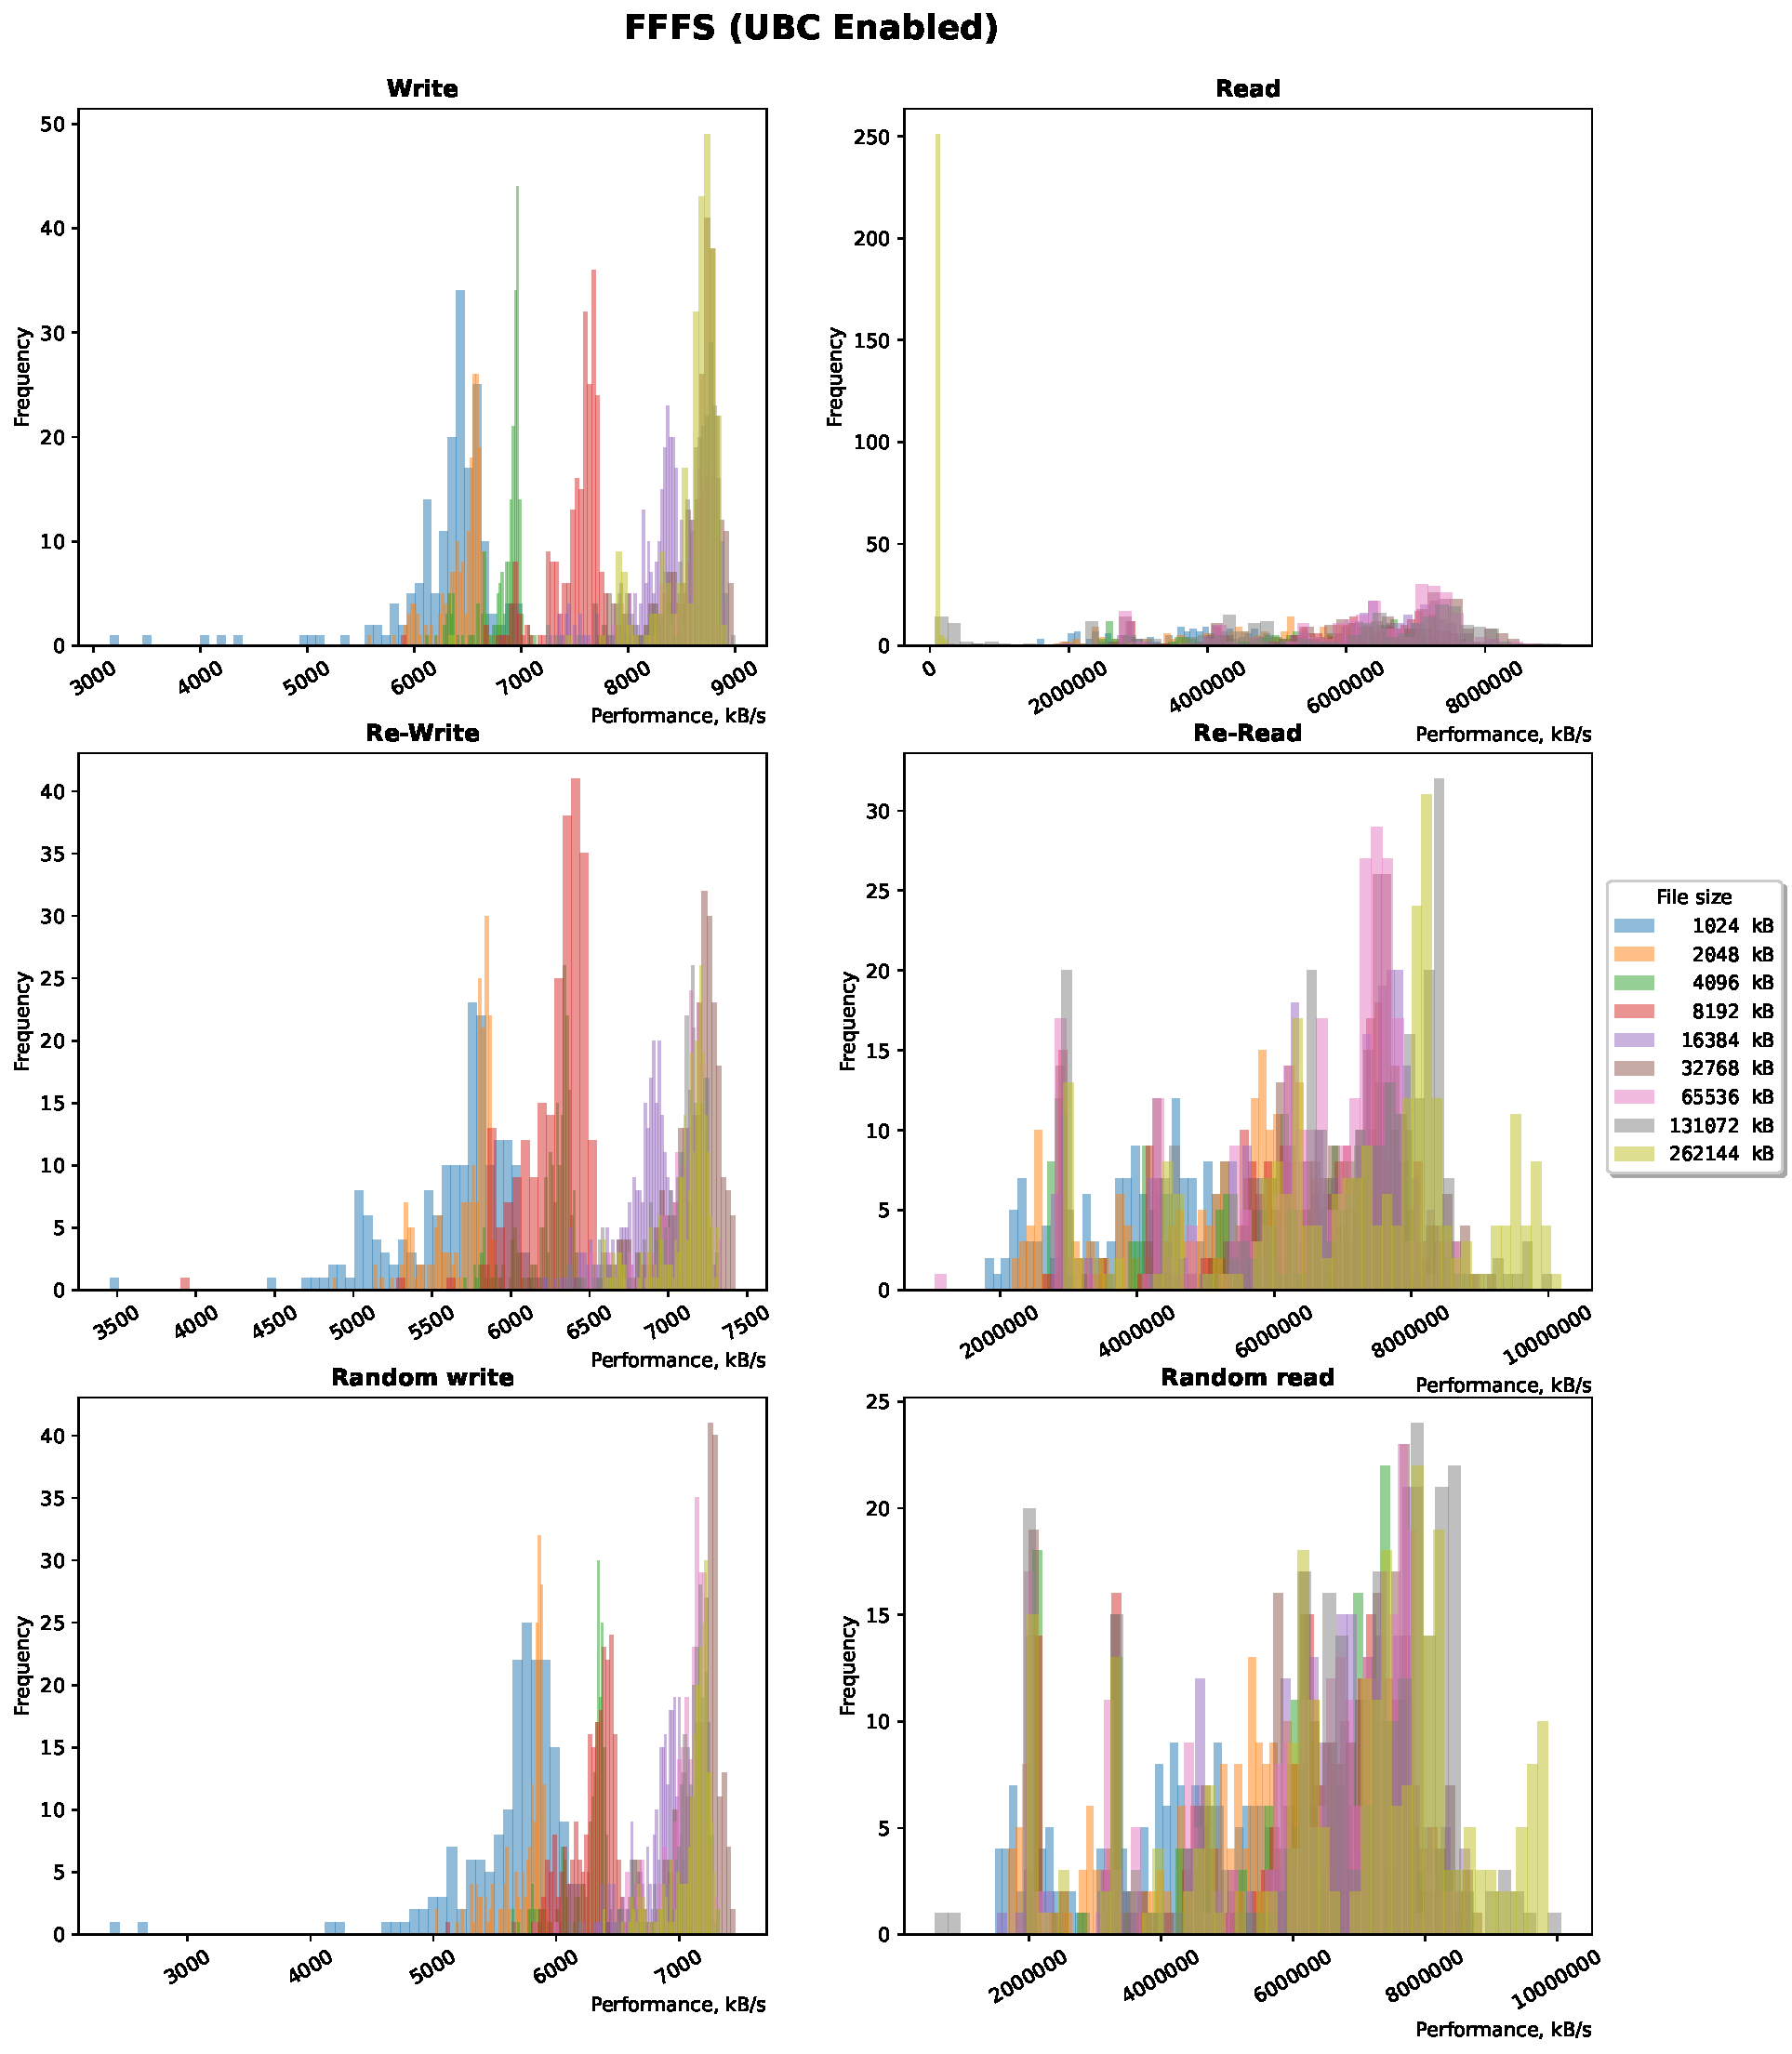
\includegraphics[width=1.0\textwidth]{figures.nosync/benchmarking/FFFS/FFFS-UBC Enabled-hist.pdf}
	\end{center}
	\caption{Performance comparison of different file sizes for FFFS with the UBC enabled}
\end{figure}

\begin{figure}[!htb]
	\label{fig:bench_fffs_without_cache}
	\begin{center}
		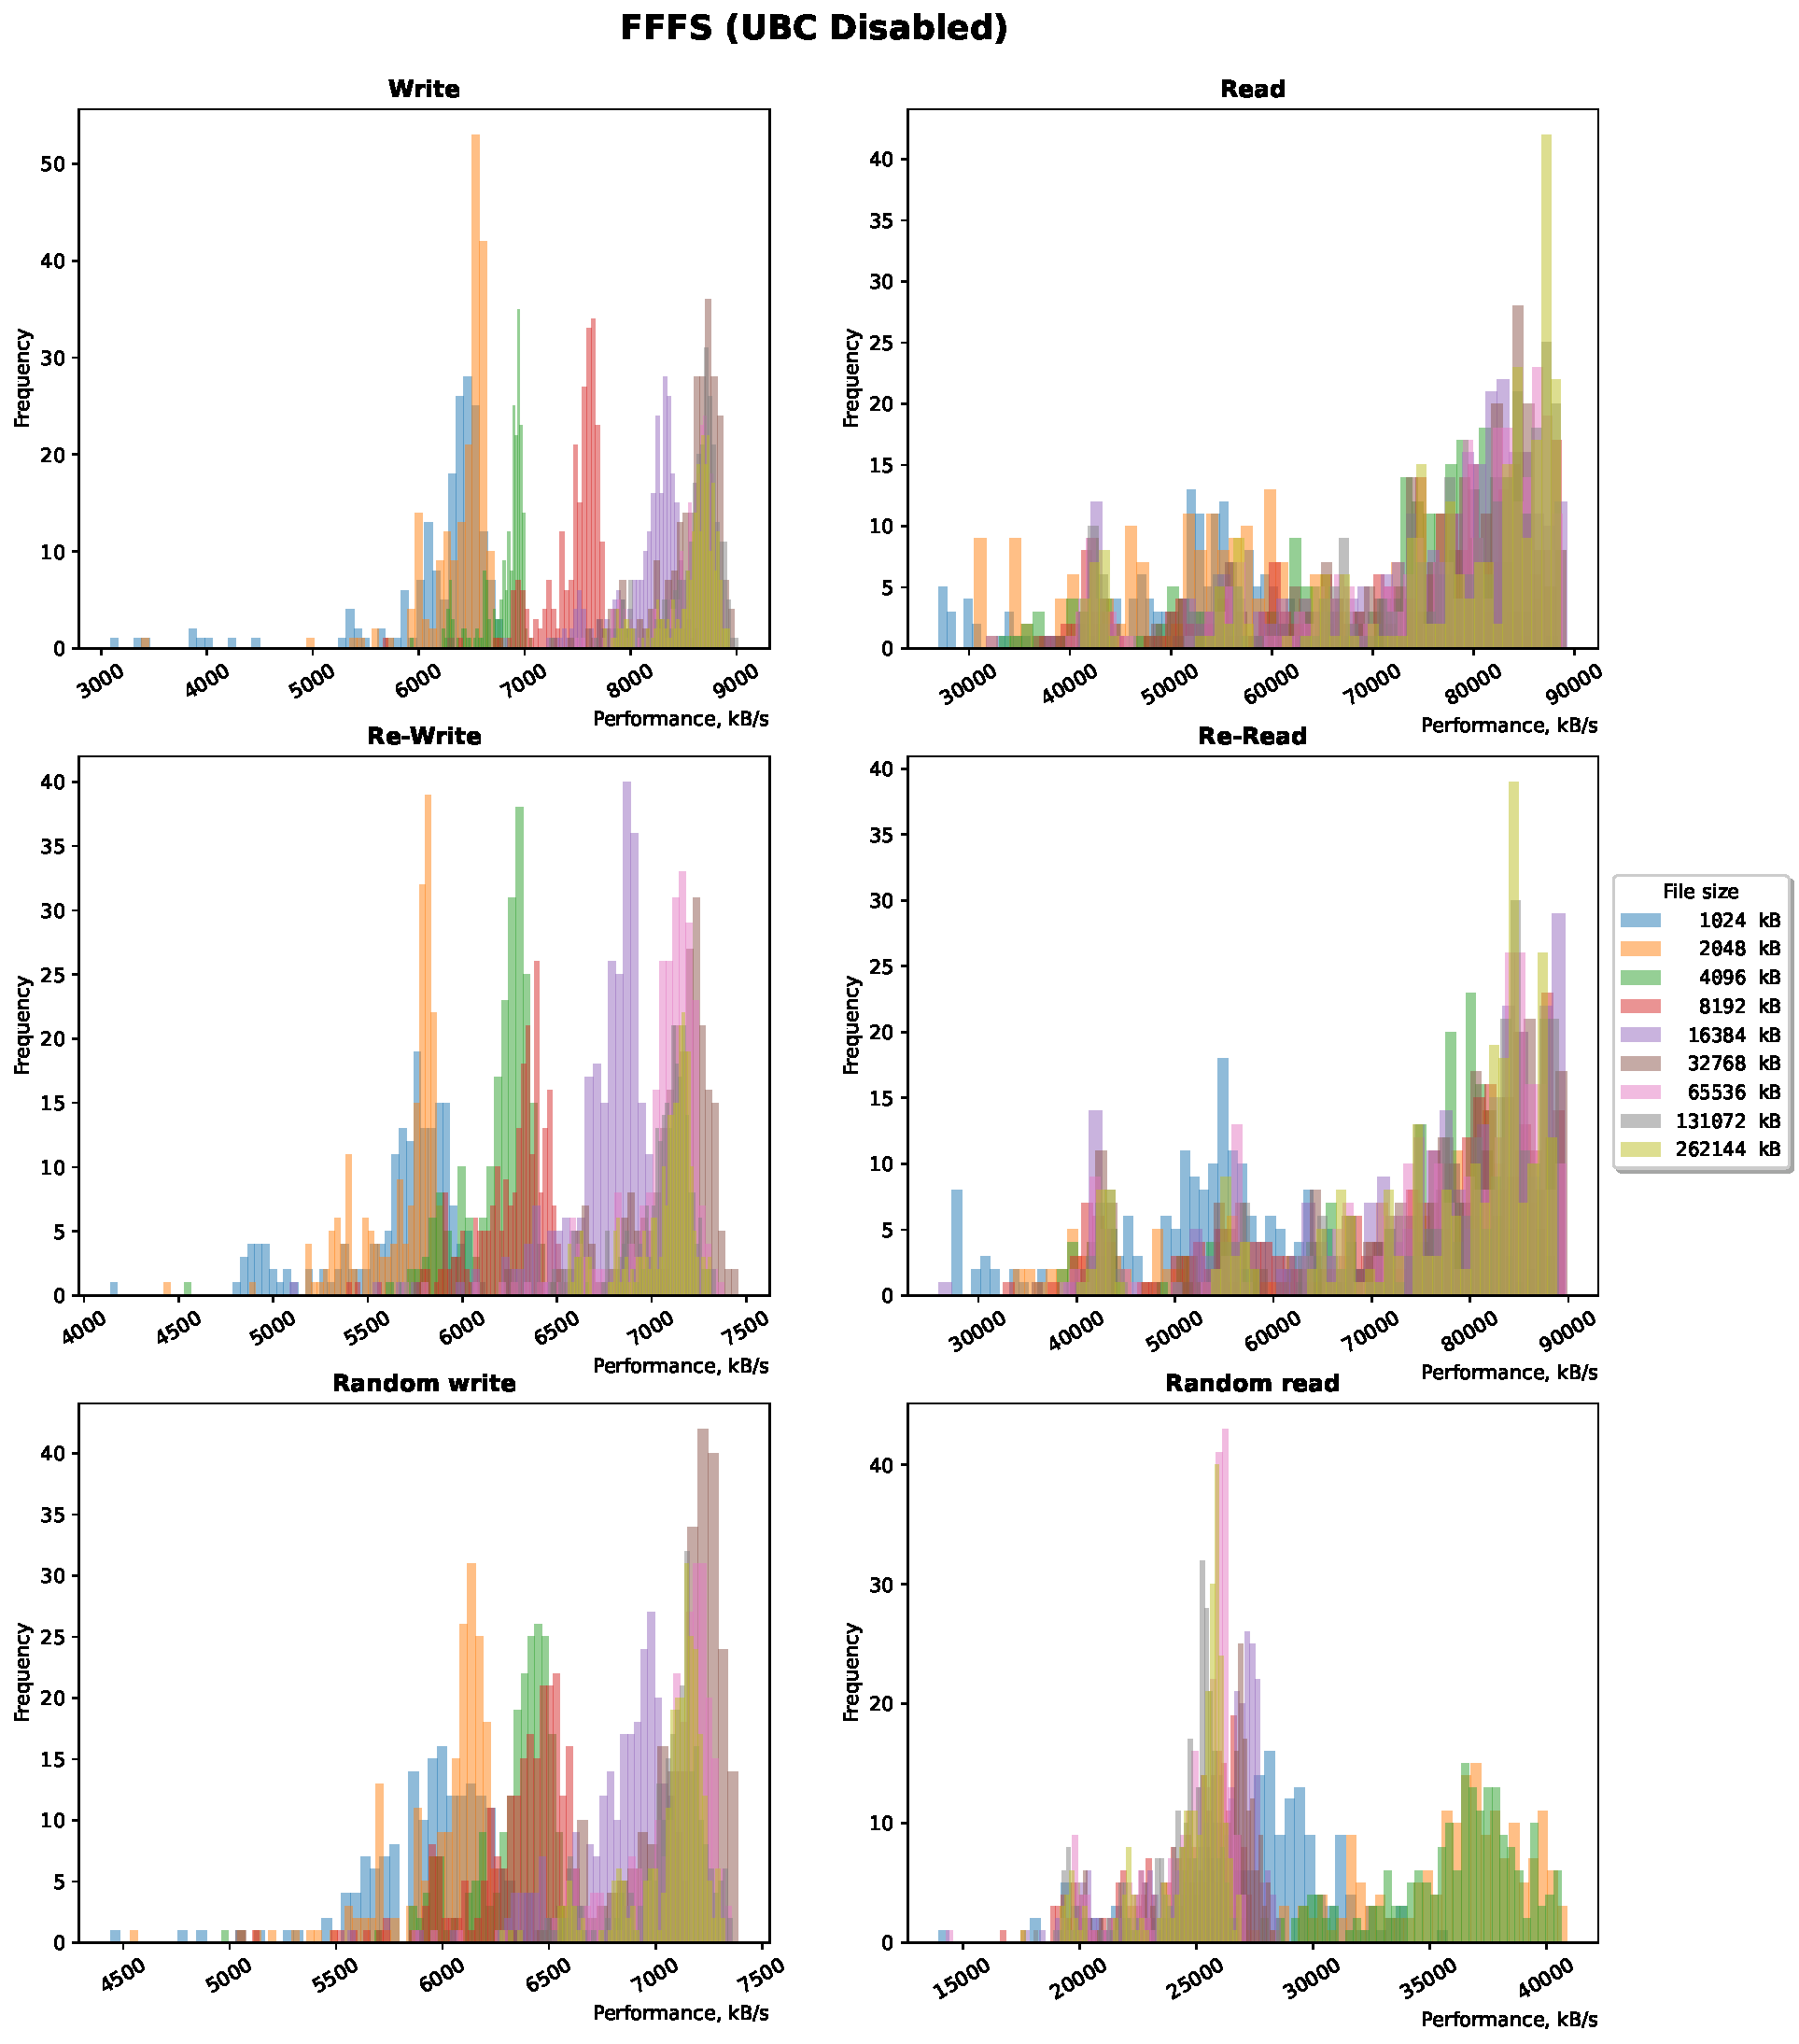
\includegraphics[width=1.0\textwidth]{figures.nosync/benchmarking/FFFS/FFFS-UBC Disabled-hist.pdf}
	\end{center}
	\caption{Performance comparison of different file sizes for FFFS with the UBC disabled}
\end{figure}




\begin{figure}[!htb]
	\label{fig:bench_apfs_with_cache}
	\begin{center}
		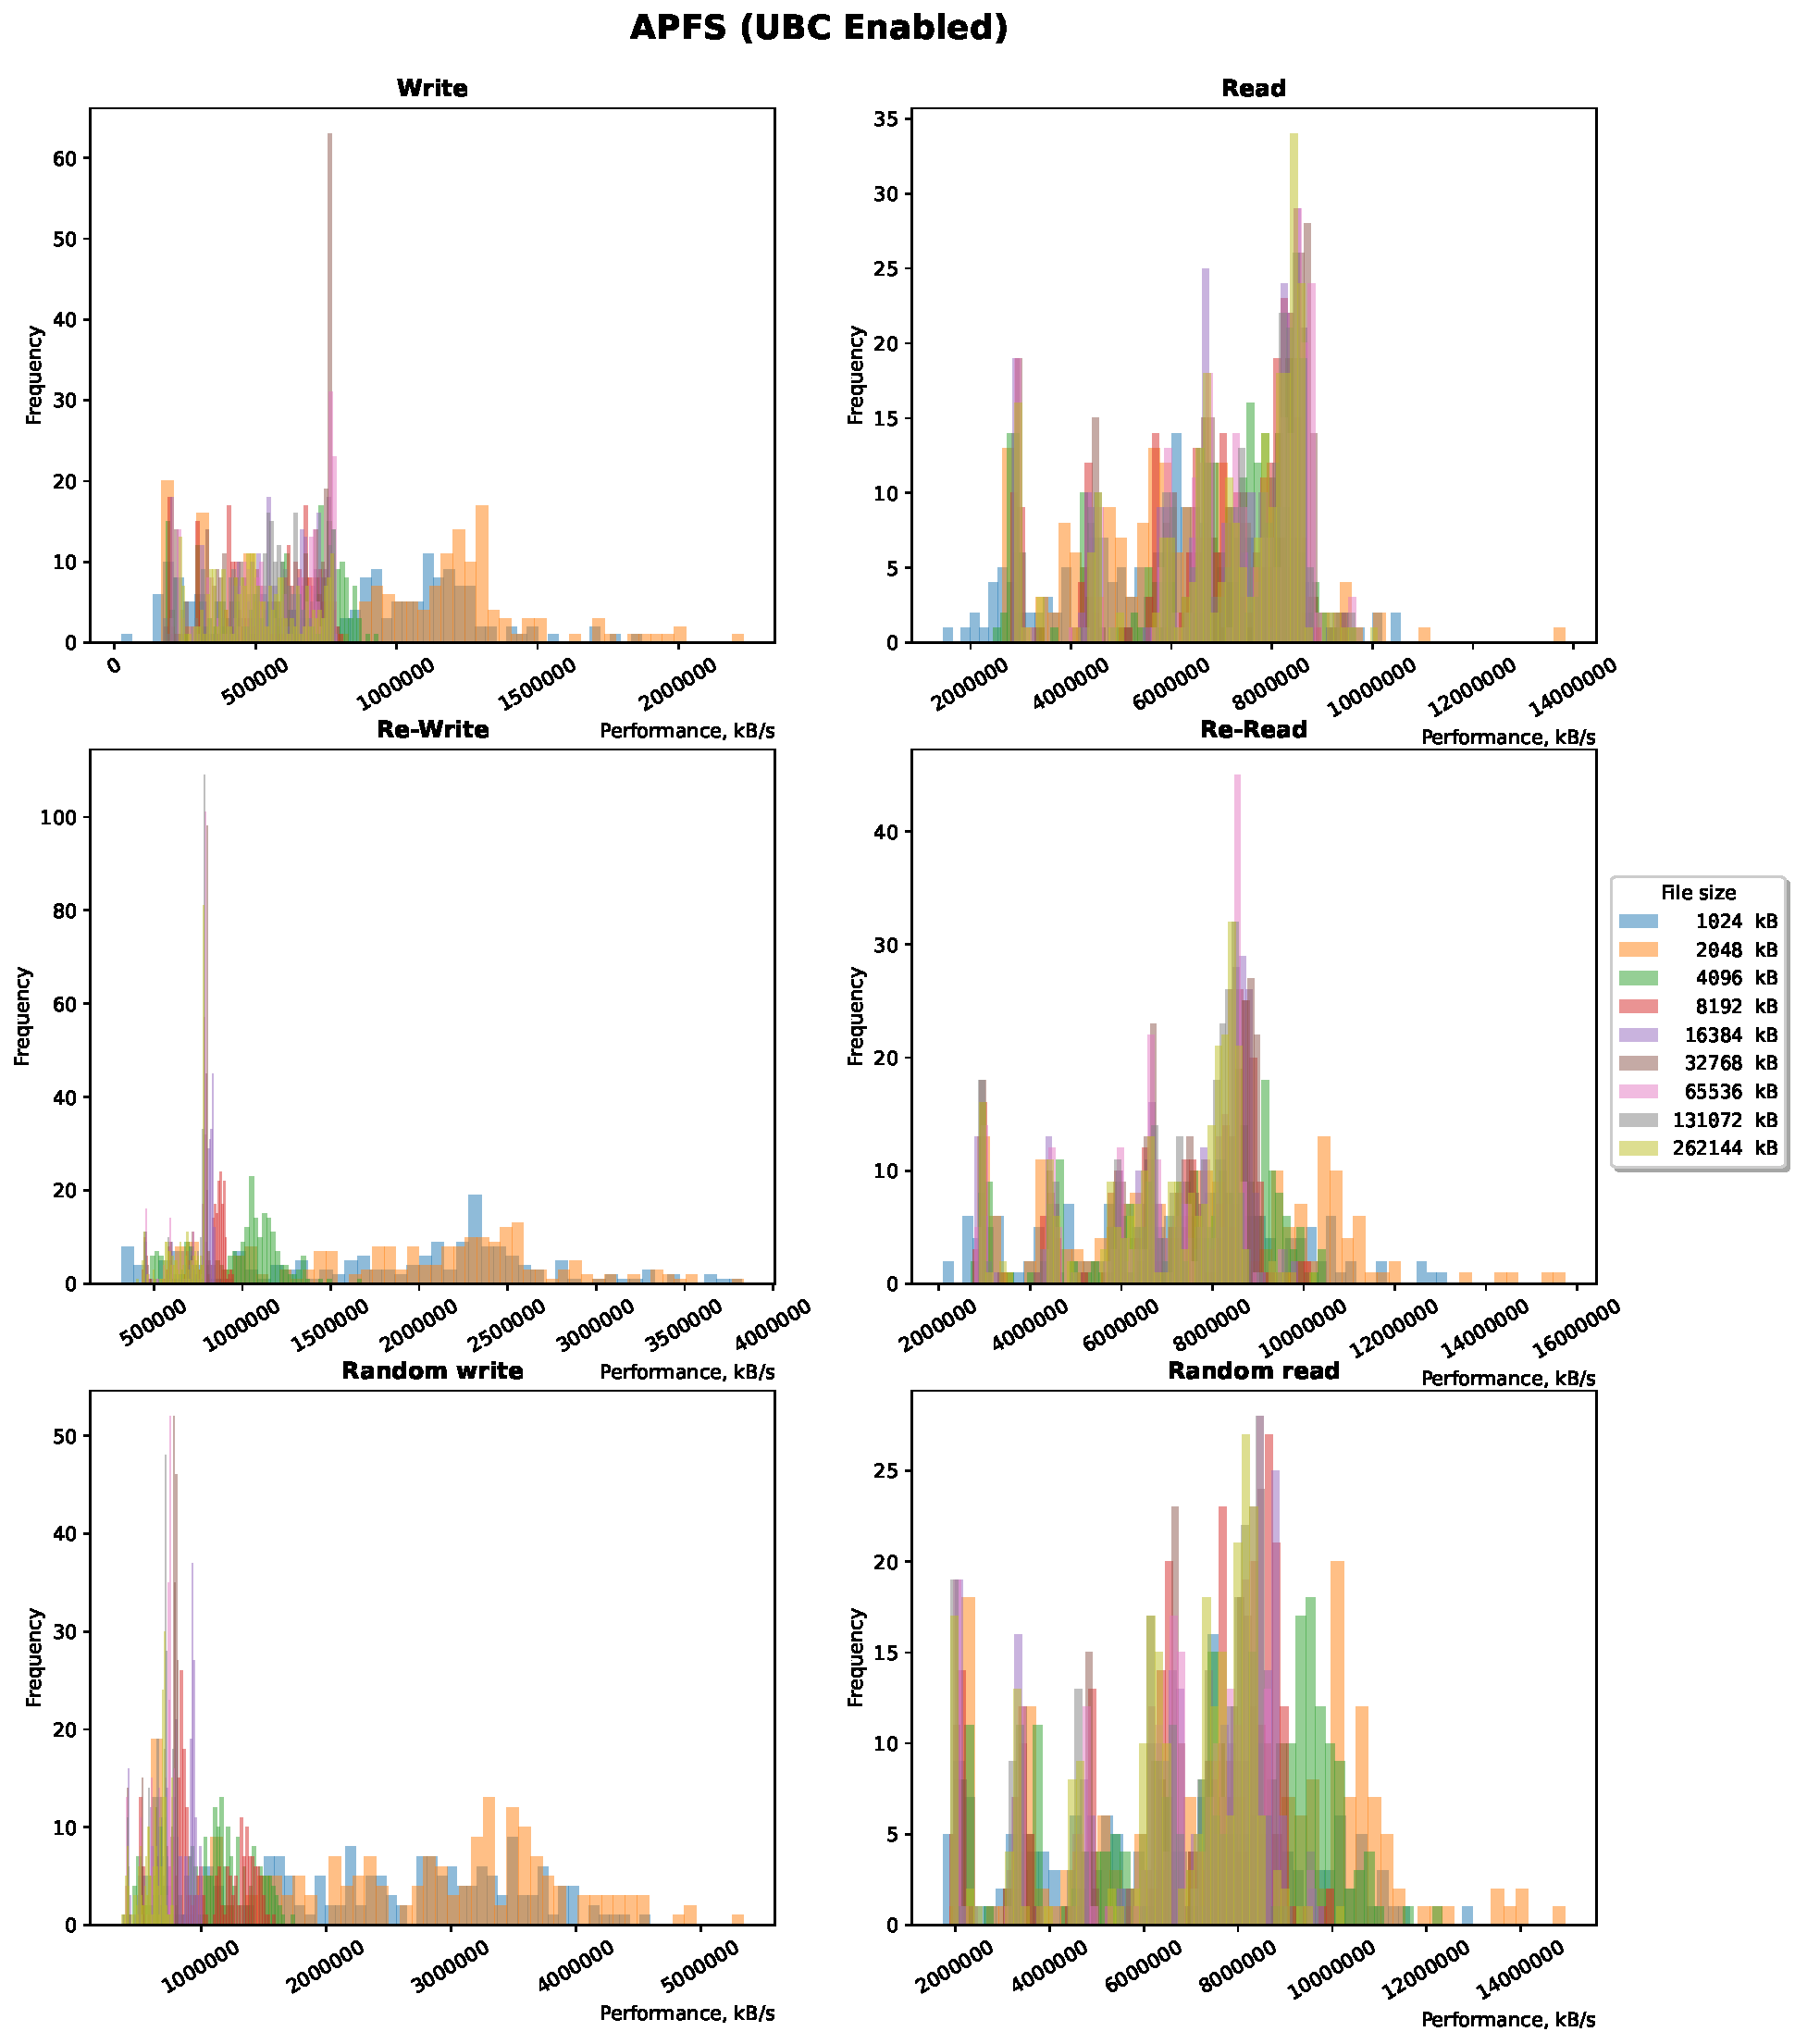
\includegraphics[width=1.0\textwidth]{figures.nosync/benchmarking/APFS/APFS-UBC Enabled-hist.pdf}
	\end{center}
	\caption{Performance comparison of different file sizes for APFS with the UBC enabled}
\end{figure}

\begin{figure}[!htb]
	\label{fig:bench_apfs_without_cache}
	\begin{center}
		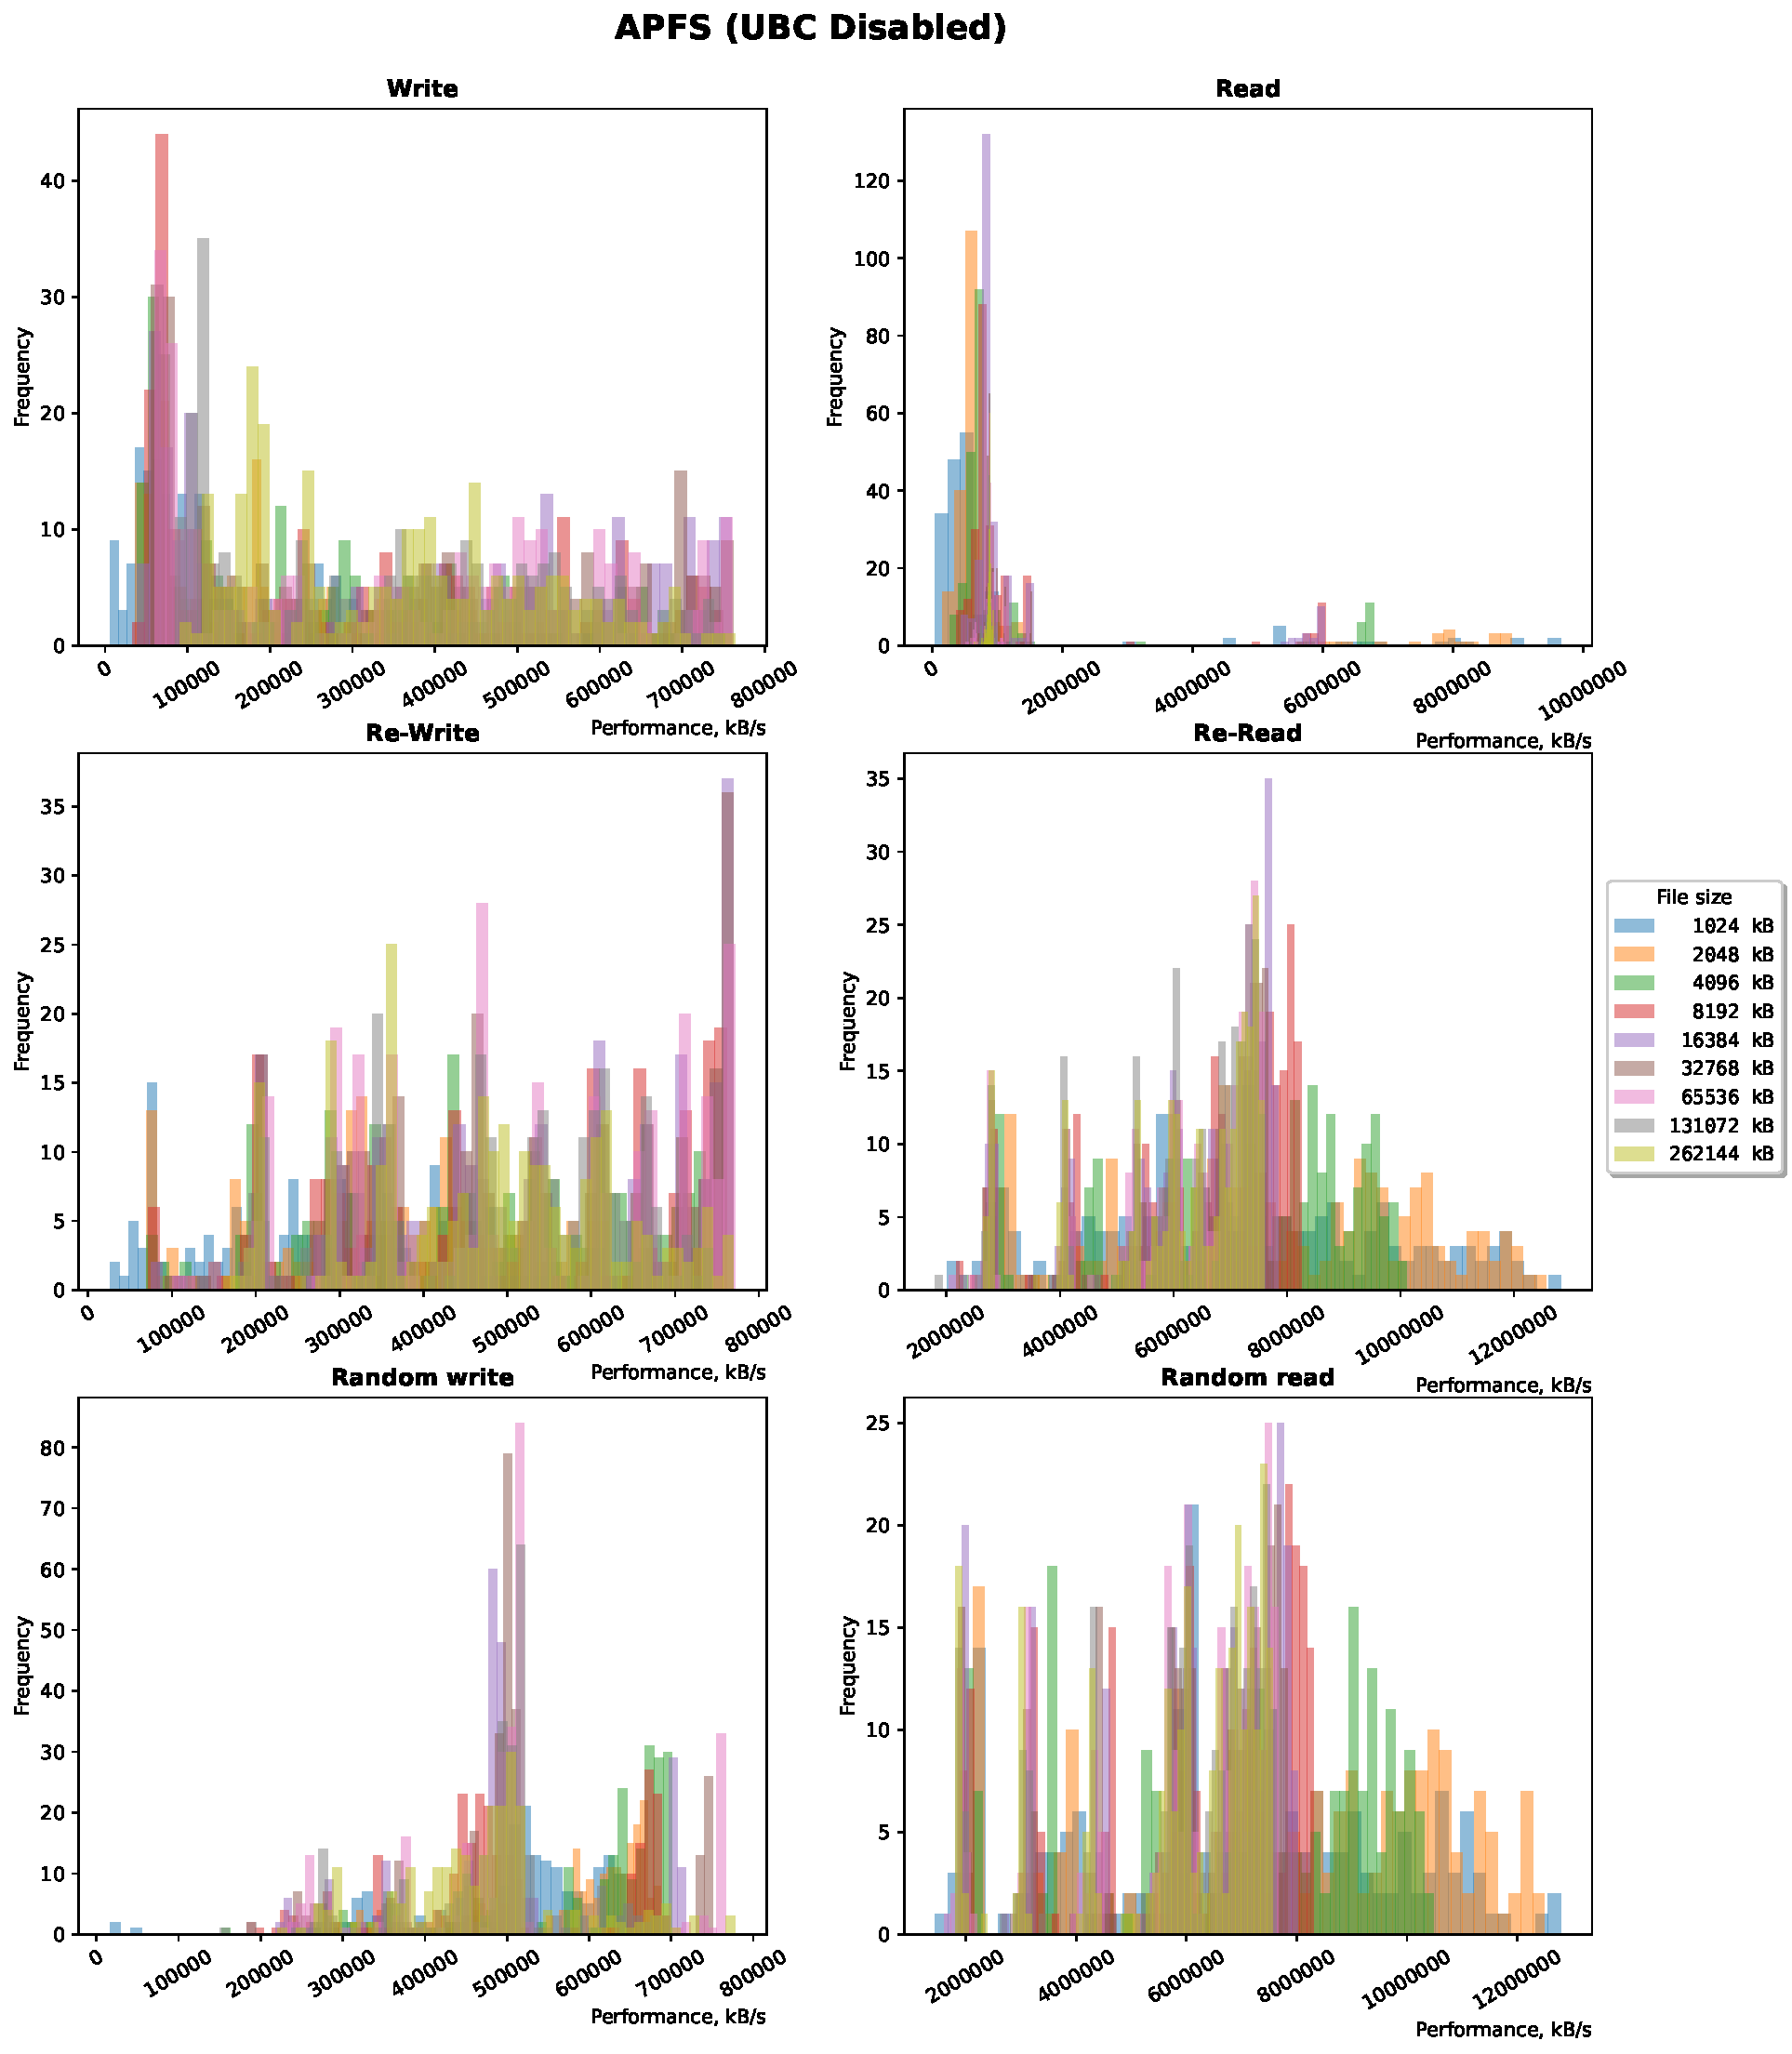
\includegraphics[width=1.0\textwidth]{figures.nosync/benchmarking/APFS/APFS-UBC Disabled-hist.pdf}
	\end{center}
	\caption{Performance comparison of different file sizes for APFS with the UBC disabled}
\end{figure}